\documentclass{beamer}

% --- Metropolis theme (modern, minimal) ---
\usetheme{metropolis}
\usepackage{appendixnumberbeamer}

\usepackage{xcolor}
\usepackage{mathrsfs}
\usepackage{amsmath} 
\usepackage{amssymb}
\usepackage{algorithm}
\usepackage{algorithmic}
\usepackage{booktabs}
\usepackage{hyperref}
\usepackage{caption}
\usepackage{graphicx}
\usepackage{subcaption} 
\usepackage{tikz}
\usetikzlibrary{shapes.geometric, arrows.meta, positioning, fit, backgrounds}
\usepackage{tcolorbox}
\tcbuselibrary{skins, breakable}
\captionsetup[figure]{font=tiny}
\graphicspath{{../../results/}}

\usepackage[
    backend=biber,
    style=alphabetic,
    sorting=ynt
]{biblatex} 
\addbibresource{bibliography.bib}
 
% --- Colour palette ---
\definecolor{CSred}{RGB}{160,32,60}
\definecolor{CSgrey}{RGB}{136,121,150}
\definecolor{CSlight}{RGB}{245,240,248}
\definecolor{alertorange}{RGB}{200,80,0}
\definecolor{metrobg}{RGB}{255,255,255}

% --- Metropolis overrides ---
\setbeamercolor{normal text}{fg=black!85, bg=metrobg}
\setbeamercolor{frametitle}{bg=CSred, fg=white}
\setbeamercolor{title separator}{fg=CSred}
\setbeamercolor{progress bar}{fg=CSred, bg=CSgrey!40}
\setbeamercolor{alerted text}{fg=CSred}
\setbeamercolor{block title}{bg=CSred, fg=white}
\setbeamercolor{block body}{bg=CSlight}
\metroset{progressbar=frametitle, sectionpage=none, numbering=fraction}
\setbeamerfont{frametitle}{series=\bfseries, size=\normalsize}

% --- tcolorbox styles ---
\tcbset{
  keybox/.style={
    colback=CSlight, colframe=CSred, fonttitle=\bfseries\small,
    boxrule=0.8pt, arc=3pt, left=5pt, right=5pt, top=4pt, bottom=4pt
  },
  warnbox/.style={
    colback=orange!7, colframe=alertorange, fonttitle=\bfseries\small,
    boxrule=0.8pt, arc=3pt, left=5pt, right=5pt, top=4pt, bottom=4pt
  },
  stressbox/.style={
    colback=CSlight, colframe=CSgrey, fonttitle=\bfseries\footnotesize,
    boxrule=0.8pt, arc=4pt, left=4pt, right=4pt, top=3pt, bottom=3pt
  } 
}

% --- Title info ---
\title{The No-U-Turn Sampler}
\subtitle{Adaptively Setting Path Lengths in Hamiltonian Monte Carlo}
\author{Adonis Jamal \quad Jean-Vincent Martini}
\institute{\'Ecole Normale Sup\'erieure Paris-Saclay --- MVA 2025--2026}
\date{March 12, 2026}

\titlegraphic{%
  \hfill
  
\includegraphics[height=1.0cm]{img/logo_ens-ps.png}
  \hspace{0.4cm}
  
\includegraphics[height=1.1cm]{img/logo_mva.jpg}
}

\begin{document}

\maketitle

% ==============================================================================
% SECTION 1: MOTIVATION
% ==============================================================================
\begin{frame}{MCMC \& Hamiltonian Monte Carlo}
    \small
    \vspace{-0.4cm}
    \begin{itemize}\setlength\itemsep{1pt}
        \item Exact posterior inference is often intractable; MCMC is asymptotically unbiased \cite{neal1993probabilistic}.
        \item Random-walk \& Gibbs \cite{metropolis1953equation,geman1984stochastic} struggle in high-dimensional or correlated spaces.
    \end{itemize}

    \vspace{-0.1cm}
    \begin{tcolorbox}[keybox, title=Hamiltonian Monte Carlo]
        \small Auxiliary momentum $r \!\sim\! \mathcal{N}(0,I)$\,+\,leapfrog: \\
        $p(\theta,r)\!\propto\!\exp\!\bigl\{\mathcal{L}(\theta)-\tfrac{1}{2}r^\top r\bigr\}$.
        Volume-preserving $\Rightarrow$ proposals can be \textbf{distant} yet \textbf{highly probable}.
    \end{tcolorbox}

      Good $L$ requires costly preliminary runs and expert knowledge, a key barrier to adoption.

    \vspace{-0.1cm}
    \noindent
    \begin{minipage}[t]{0.49\textwidth}
      \begin{tcolorbox}[warnbox, title=Step size $\varepsilon$]
        \footnotesize
        Too small $\Rightarrow$ wasted computation\\[2pt]
        Too large $\Rightarrow$ high rejection rate
      \end{tcolorbox}
    \end{minipage}
    \hfill
    \begin{minipage}[t]{0.49\textwidth}
      \begin{tcolorbox}[warnbox, title=Leapfrog steps $L$]
        \footnotesize
        Too small $\Rightarrow$ random walk \\[2pt]
        Too large $\Rightarrow$ trajectory loops back
      \end{tcolorbox}
    \end{minipage}
    \vspace*{-0.1cm}
    {\small \textbf{NUTS addresses both tuning problems simultaneously.}}
\end{frame}

% ==============================================================================
% SECTION 2: NUTS METHODOLOGY
% ==============================================================================
\begin{frame}{NUTS Methodology}
  \small
  \vspace{-0.2cm}
  \begin{tcolorbox}[keybox, title={No-U-Turn criterion}]
    \footnotesize
    Stop when the trajectory doubles back: $(\theta^+ \!-\! \theta^-)\!\cdot\! r^- \!<\! 0$ \;or\; $(\theta^+ \!-\! \theta^-)\!\cdot\! r^+ \!<\! 0$.
  \end{tcolorbox}

  \vspace{-0.1cm}
  \noindent
  \begin{minipage}[t]{0.48\textwidth}
    \textbf{Recursive doubling}
    \begin{enumerate}\setlength\itemsep{0pt}
      \footnotesize
      \item Draw direction $v_j \!\sim\! \mathrm{Unif}(\{-1,+1\})$
      \item Take $2^j$ leapfrog steps of size $v_j\varepsilon$
      \item Grow balanced binary tree; halt on U-turn
    \end{enumerate}
    \vspace{0.05cm}
    {\footnotesize Memory $\mathcal{O}(2^j)\!\to\!\mathcal{O}(j)$: partition $\mathcal{C}\!=\!\mathcal{C}^{\mathrm{old}}\!\cup\!\mathcal{C}^{\mathrm{new}}$, propose $w'\!\in\!\mathcal{C}^{\mathrm{new}}$, accept with $\min\!\bigl(1,\frac{|\mathcal{C}^{\mathrm{new}}|}{|\mathcal{C}^{\mathrm{old}}|}\bigr)$.}
  \end{minipage}
  \hfill
  \begin{minipage}[t]{0.48\textwidth}
    \textbf{Dual averaging} {\footnotesize (warm-up only)}\\[2pt]
    {\footnotesize Drive acceptance to target $\delta$:}
    \vspace{-0.2cm}
    {\footnotesize\[x_{t+1} \!=\! \mu - \frac{\sqrt{t}}{\gamma(t+t_0)}\!\sum_{i=1}^{t}\!H_i,\]}
    {\footnotesize\[\bar{x}_{t+1} = t^{-\kappa}x_{t+1} + (1-t^{-\kappa})\bar{x}_t\]}
    \vspace{-0.45cm}
    {\footnotesize
    $x\!=\!\log\varepsilon$,\; $\mu\!=\!\log (10\varepsilon_0)$\\[10pt]
    Fixed Hyperparams: $\gamma\!=\!0.05$, $t_0\!=\!10$, $\kappa\!=\!0.75$}
  \end{minipage}

  \vspace{0.1cm}
  \begin{tcolorbox}[keybox]
    \small No-U-Turn criterion + dual averaging $\Rightarrow$ NUTS is \textbf{entirely tuning-free}.
  \end{tcolorbox}
\end{frame}

% ==============================================================================
% SECTION 4: IMPLEMENTATION AND BENCHMARKS
% ==============================================================================
\begin{frame}{Evaluating NUTS: The Paper's Benchmarks}
  \vspace{-0.2cm}
    The paper tests NUTS on four \textbf{unimodal or mildly structured} targets.

    \vspace{-0.05cm}
    \noindent
    \begin{minipage}[t]{0.22\textwidth}\centering
      \begin{tcolorbox}[stressbox, title=250-D, halign=center]
        \footnotesize Multivariate Normal
      \end{tcolorbox}
    \end{minipage}
    \hfill
    \begin{minipage}[t]{0.22\textwidth}\centering
      \begin{tcolorbox}[stressbox, title=25-D, halign=center]
        \footnotesize Logistic Regression
      \end{tcolorbox}
    \end{minipage}
    \hfill
    \begin{minipage}[t]{0.22\textwidth}\centering
      \begin{tcolorbox}[stressbox, title=302-D, halign=center]
        \footnotesize Hierarchical LR
      \end{tcolorbox}
    \end{minipage}
    \hfill
    \begin{minipage}[t]{0.22\textwidth}\centering
      \begin{tcolorbox}[stressbox, title=3001-D, halign=center]
        \footnotesize Stochastic Volatility
      \end{tcolorbox}
    \end{minipage}

    \vspace{-0.3cm}
    \begin{tcolorbox}[keybox]
      NUTS matches or exceeds best-tuned HMC on \textbf{all four benchmarks} without any trajectory-length tuning. What about posteriors with complex geometry?
    \end{tcolorbox}

      \small
  \vspace{-0.25cm}
  % TikZ diagram of three pathologies
  \begin{center}
  \begin{tikzpicture}[>=Stealth, font=\footnotesize]

    % Box 1: Multimodality
    \node[draw=CSred, fill=CSlight, rounded corners=4pt, inner sep=5pt,
          text width=2.4cm, align=center] (A) {
      \textbf{Multimodality}\\[2pt]
      \begin{tikzpicture}[scale=0.32]
        \fill[CSred!70] (-2.4, 0) ellipse (0.28 and 0.6);
        \fill[CSred!70] (0,    0) ellipse (0.28 and 0.6);
        \fill[CSred!70] (2.4,  0) ellipse (0.28 and 0.6);
        \draw[->, gray, thin] (-3.1,0) -- (3.1,0);
      \end{tikzpicture}\\[1pt]
      {\scriptsize BNN, 191-D\\$5!\!\times\!5!=14400$ modes}
    };

    % Box 2: Dense correlations
    \node[draw=CSred, fill=CSlight, rounded corners=4pt, inner sep=5pt,
          text width=2.8cm, align=center, right=0.3cm of A] (B) {
      \textbf{Dense Correlations}\\[2pt]
      
\begin{tikzpicture}[scale=0.32]
        \foreach \i in {1,...,4}{
          \foreach \j in {1,...,4}{
            \pgfmathsetmacro\op{0.15 + 0.7*exp(-0.4*abs(\i-\j))}
            \fill[CSred, opacity=\op]
              ({-0.9+(\i-1)*0.6}, {0.9-(\j-1)*0.6}) rectangle
              ({-0.9+(\i-1)*0.6+0.55}, {0.9-(\j-1)*0.6-0.55});
          }
        }
      \end{tikzpicture}\\[1pt]
      {\scriptsize GP Classif., 150-D\\dense $150\!\times\!150$ cov.}
    };

    % Box 3: Funnel
    \node[draw=CSred, fill=CSlight, rounded corners=4pt, inner sep=5pt,
          text width=2.8cm, align=center, right=0.3cm of B] (C) {
      \textbf{Varying Geometry}\\[2pt]
      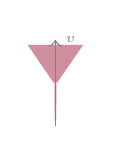
\begin{tikzpicture}[scale=0.32]
        \fill[CSred!50]
          (0, 1.5) -- (-1.1, 1.5) -- (-0.07, 0) -- (0.07, 0) -- (1.1, 1.5) -- cycle;
        \fill[CSred!20]
          (-0.07,0) -- (0.07,0) -- (0.04,-1.5) -- (-0.04,-1.5) -- cycle;
        \draw[->, gray, thin] (0,-1.7) -- (0,1.7) node[right]{\tiny $v$};
      \end{tikzpicture}\\[1pt]
      {\scriptsize Neal's Funnel, 10-D\\spatially varying $\sigma$}
    };

  \end{tikzpicture}
  \end{center}
\end{frame}


% ==============================================================================
% SECTION 5: STRESS TESTS
% ==============================================================================
\begin{frame}{Beyond the Paper: Three Stress Tests}
  \vspace{-0.3cm}
  \begin{tcolorbox}[warnbox, title=Results]
    \footnotesize
    \begin{itemize}\setlength\itemsep{2pt}
      \item \textbf{BNN:} NUTS explores wider weight space but lower ESS/grad than well-tuned HMC ($0.03$ vs.\ $1.57\!\times\!10^{-4}$).
      \item \textbf{GPC:} Modest 40\% ESS/grad gain, but NUTS uses $4\times$ more gradient evaluations; advantage is narrow.
      \item \textbf{Funnel:} NUTS recovers $\mathrm{Var}(v)\!\approx\!9$ (truth); HMC's fixed $\varepsilon$ fails to explore the neck.
    \end{itemize}
    {\footnotesize Adaptive trajectory length is critical on complex posteriors.}
  \end{tcolorbox}
  
  \vspace{-0.3cm}
  \begin{figure}[htbp]
    \centering
    \begin{subfigure}[t]{0.42\textwidth}
        \centering
        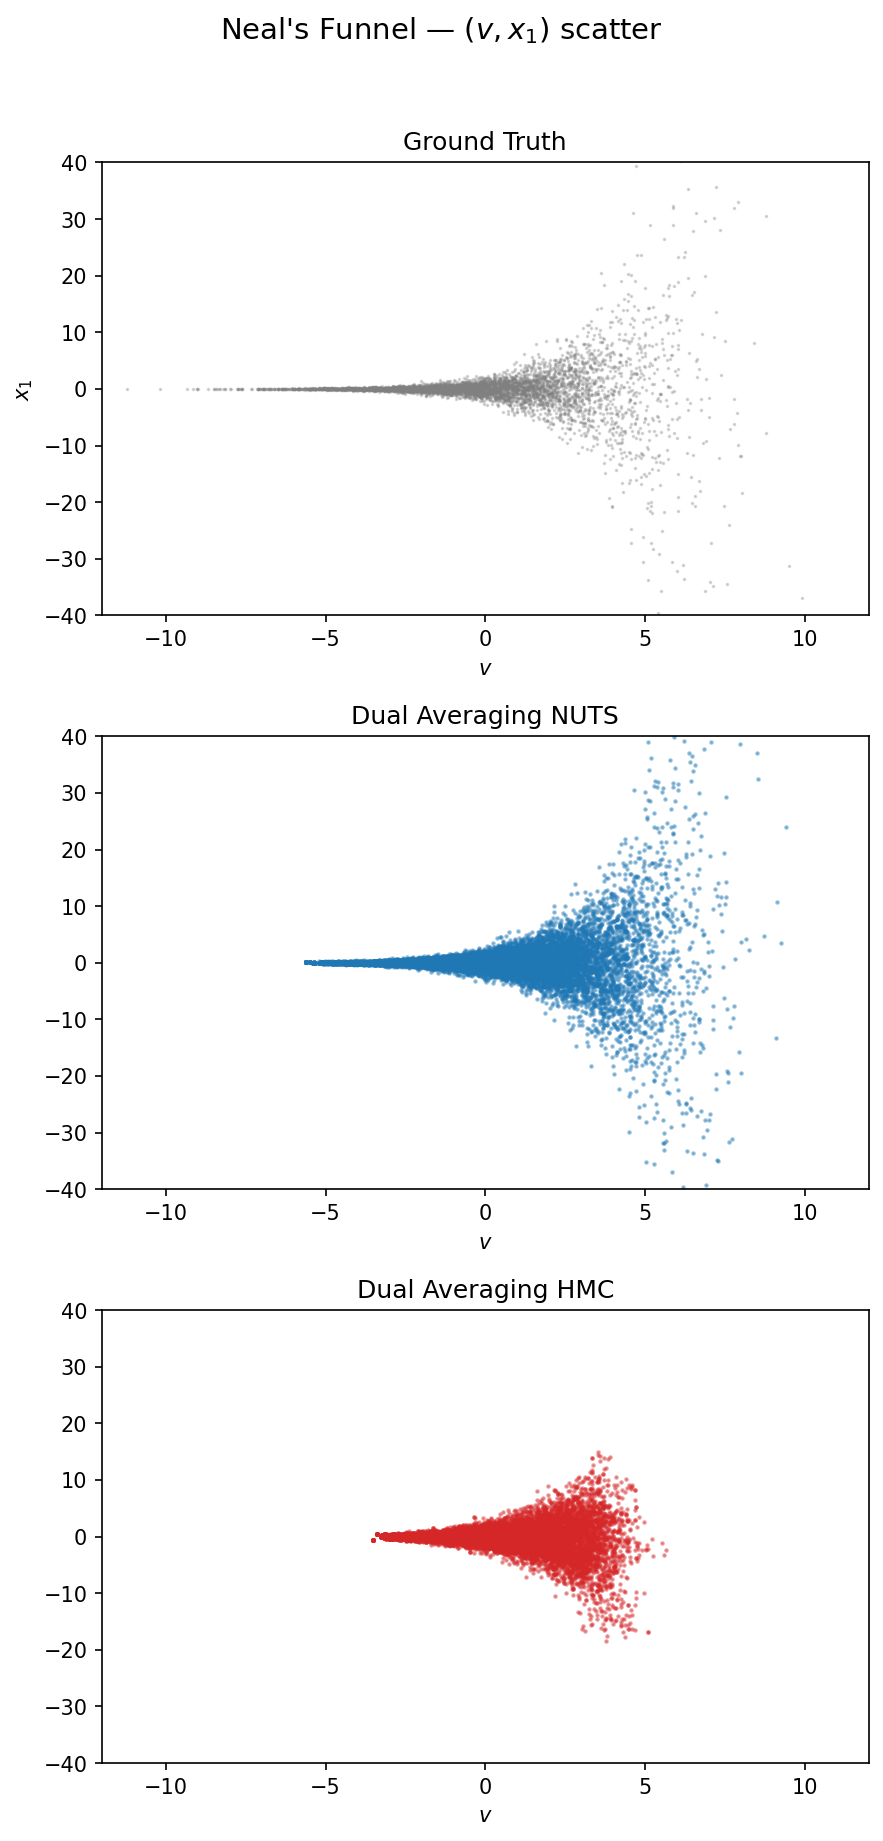
\includegraphics[width=0.38\textwidth]{Funnel/funnel_scatter_vertical.png}
        \label{fig:funnel_scatter}
    \end{subfigure}
    \hfill
    \begin{subfigure}[t]{0.55\textwidth}
        \centering
        
\includegraphics[width=0.7\textwidth]{Funnel/trace_plots.png}
        \label{fig:funnel_traces}
    \end{subfigure}
    \vspace{-0.2cm}
    \label{fig:funnel_diagnostics}
\end{figure} 

  
\end{frame}

% ==============================================================================
% SECTION 6: CONCLUSION
% ==============================================================================

\begin{frame}{Summary \& Contributions}
  \vspace*{-0.2cm}
  \scriptsize
  \begin{tcolorbox}[warnbox, title=Paper assessment]
    \begin{itemize}\setlength\itemsep{0.05pt}
      \item[\textcolor{green!60!black}{\textbf{+}}] Resolves HMC's central practical limitation; conceptually simple yet theoretically rigorous
      \item[\textcolor{green!60!black}{\textbf{+}}] No-U-Turn criterion + recursive doubling preserve detailed balance
      \item[\textcolor{green!60!black}{\textbf{+}}] Dual averaging for step-size adaptation $\Rightarrow$ essentially tuning-free
      \item[\textcolor{red!70!black}{\textbf{--}}] Dual-averaging hyperparameters justified empirically; robustness across geometries is open
      \item[\textcolor{red!70!black}{\textbf{--}}] Performance guarantees mainly asymptotic; limited range of posterior geometries tested
    \end{itemize} 
  \end{tcolorbox}

  \vspace{-0.1cm}
  \begin{tcolorbox}[keybox, title=Our contributions]
    \begin{itemize}\setlength\itemsep{0.05pt}
      \item \textbf{Proofs} of uniform $\mathcal{C}$ distribution and detailed balance of the memory-efficient kernel (only sketched in paper)
      \item \textbf{Reproduced} all 4 benchmarks; NUTS matches or exceeds best-tuned HMC without trajectory-length tuning
      \item \textbf{Stress tests:} adaptive trajectory length is critical on complex posteriors, the gains are most dramatic on Funnel \& BNN; advantage narrows on dense GP
      \item \textbf{Conclusion:} confirms NUTS's suitability as a general-purpose inference engine for modern Bayesian models
    \end{itemize}
  \end{tcolorbox}
\end{frame}


% ==============================================================================
% BIBLIOGRAPHY
% ==============================================================================
\begingroup
\setbeamertemplate{footline}{} 

\begin{frame}[allowframebreaks, noframenumbering]{Bibliography}
    \printbibliography[heading=none]
\end{frame}
\endgroup

% ==============================================================================
% APPENDIX
% ==============================================================================
\appendix

\begin{frame}{Appendix: The Transition Kernel \& Detailed Balance}
    To reduce memory from $\mathcal{O}(2^j)$ to $\mathcal{O}(j)$, NUTS partitions the candidate set: $\mathcal{C} = \mathcal{C}^{\text{old}} \cup \mathcal{C}^{\text{new}}$.

    \vspace{0.03cm}
    \textbf{The Proposal:}
    \begin{itemize}
        \item From state $w \in \mathcal{C}^{\text{old}}$, propose a jump to $w' \in \mathcal{C}^{\text{new}}$ uniformly.
        \item Accept with probability: $\min\left(1, \frac{|\mathcal{C}^{\text{new}}|}{|\mathcal{C}^{\text{old}}|}\right)$
    \end{itemize}

    \vspace{0.03cm}
    \begin{tcolorbox}[colback=CSlight, colframe=CSgrey, title=Proof of Detailed Balance (Intuition)]
        We must satisfy: $p(w|\mathcal{C})T(w'|w, \mathcal{C}) = p(w'|\mathcal{C})T(w|w', \mathcal{C})$
        
        \vspace{0.05cm}
        Substituting the prior $p(w|\mathcal{C}) = \frac{1}{|\mathcal{C}|}$ and the acceptance rates:
        $$ \frac{1}{|\mathcal{C}||\mathcal{C}^{\text{new}}|} \min\left(1, \frac{|\mathcal{C}^{\text{new}}|}{|\mathcal{C}^{\text{old}}|}\right) = \frac{1}{|\mathcal{C}||\mathcal{C}^{\text{old}}|} \min\left(1, \frac{|\mathcal{C}^{\text{old}}|}{|\mathcal{C}^{\text{new}}|}\right) $$
        Proving the kernel preserves the target distribution.
    \end{tcolorbox}
\end{frame}


\begin{frame}{Appendix: Uniform Distribution over the Candidate Set}
    \small
    \textbf{Claim:} $p(w \mid u,\mathcal{B},\mathcal{C},\varepsilon) = \tfrac{1}{|\mathcal{C}|}\,\mathbb{I}[w\in\mathcal{C}]$

    Let $w=(\theta,r)$. The augmented joint density is
    $p(\theta,r,u) \propto \mathbb{I}\!\left[u \le \exp\!\left(\mathcal{L}(\theta)-\tfrac12 r\cdot r\right)\right].$

    Conditioning on $(u,\mathcal{B},\mathcal{C},\varepsilon)$:
    \begin{equation*}
      p(w \mid u,\mathcal{B},\mathcal{C},\varepsilon) \propto
      \underbrace{p(\mathcal{B},\mathcal{C}\mid w,u,\varepsilon)}_{\text{(ii)}} \cdot
      \underbrace{p(w\mid u)}_{\text{(i)}}
    \end{equation*}

    \begin{tcolorbox}[colback=CSlight, colframe=CSgrey, fonttitle=\bfseries\footnotesize,
      boxrule=0.8pt, arc=3pt, left=4pt, right=4pt, top=3pt, bottom=3pt]
      \footnotesize
      \textbf{(i)} \textbf{C.3}: $w\in\mathcal{C}$ implies the slice constraint holds $\Rightarrow$
      $p(w\mid u) \propto 1$ on $\mathcal{C}$.\\[3pt]
      \textbf{(ii)} \textbf{C.2}: current state $\in\mathcal{C}$;\quad
      \textbf{C.4}: probability of generating $(\mathcal{B},\mathcal{C})$ is the same for all $w\in\mathcal{C}$ $\Rightarrow$ $p(\mathcal{B},\mathcal{C}\mid w,u,\varepsilon) \propto \mathbb{I}[w\in\mathcal{C}]$.
    \end{tcolorbox}

    Substituting: $p(w \mid u,\mathcal{B},\mathcal{C},\varepsilon) \propto \mathbb{I}[w\in\mathcal{C}]$, i.e.\ uniform over $\mathcal{C}$.

    By \textbf{C.1} (leapfrog is volume-preserving), all elements of $\mathcal{C}$ carry equal mass:
    \[
      p(w \mid u,\mathcal{B},\mathcal{C},\varepsilon) = \frac{1}{|\mathcal{C}|}\,\mathbb{I}[w\in\mathcal{C}]. \qquad \square
    \]
\end{frame}

\begin{frame}{Heuristic for Initial Epsilon}
    \setcounter{algorithm}{3} % Sets the algorithm counter so it displays as Algorithm 4
    
    \begin{algorithm}[H]
    \caption{Heuristic for choosing an initial value of $\epsilon$}
    \begin{algorithmic}
    \STATE \textbf{function} $\text{FindReasonableEpsilon}(\theta)$
    \STATE Initialize $\epsilon = 1, r \sim \mathcal{N}(0, I)$. ($I$ denotes the identity matrix.)
    \STATE Set $\theta', r' \gets \text{Leapfrog}(\theta, r, \epsilon)$.
    \STATE $a \gets 2\mathbb{I}\left[\frac{p(\theta', r')}{p(\theta, r)} > 0.5\right] - 1$.
    \WHILE{$\left(\frac{p(\theta', r')}{p(\theta, r)}\right)^a > 2^{-a}$}
        \STATE $\epsilon \gets 2^a \epsilon$.
        \STATE Set $\theta', r' \gets \text{Leapfrog}(\theta, r, \epsilon)$.
    \ENDWHILE
    \STATE \textbf{return} $\epsilon$.
    \end{algorithmic}
    \end{algorithm}
\end{frame}

\begin{frame}{Hamiltonian Monte Carlo}
    \setcounter{algorithm}{4} % Sets the algorithm counter so it displays as Algorithm 5
    
    \begin{algorithm}[H]
    \footnotesize % Reduces font size slightly to ensure it fits on the presentation slide
    \caption{Hamiltonian Monte Carlo with Dual Averaging}
    \begin{algorithmic}
    \STATE Given $\theta^0$, $\delta$, $\lambda$, $\mathcal{L}$, $M$, $M^{\text{adapt}}$:
    \STATE Set $\epsilon_0 = \text{FindReasonableEpsilon}(\theta), \mu = \log(10\epsilon_0), \bar{\epsilon}_0 = 1, \bar{H}_0 = 0, \gamma = 0.05, t_0 = 10, \kappa = 0.75$.
    \FOR{$m = 1$ to $M$}
        \STATE Reample $r^0 \sim \mathcal{N}(0, I)$.
        \STATE Set $\theta^m \gets \theta^{m-1}, \tilde{\theta} \gets \theta^{m-1}, \tilde{r} \gets r^0, L_m = \max\{1, \text{Round}(\lambda/\epsilon_{m-1})\}$.
        \FOR{$i = 1$ to $L_m$}
            \STATE Set $\tilde{\theta}, \tilde{r} \gets \text{Leapfrog}(\tilde{\theta}, \tilde{r}, \epsilon_{m-1})$.
        \ENDFOR
        \STATE With probability $\alpha = \min \left\{1, \frac{\exp\{\mathcal{L}(\tilde{\theta}) - \frac{1}{2}\tilde{r} \cdot \tilde{r}\}}{\exp\{\mathcal{L}(\theta^{m-1}) - \frac{1}{2}r^0 \cdot r^0\}}\right\}$, set $\theta^m \gets \tilde{\theta}, r^m \gets -\tilde{r}$.
        \IF{$m \leq M^{\text{adapt}}$}
            \STATE Set $\bar{H}_m = \left(1 - \frac{1}{m+t_0}\right) \bar{H}_{m-1} + \frac{1}{m+t_0}(\delta - \alpha)$.
            \STATE Set $\log \epsilon_m = \mu - \frac{\sqrt{m}}{\gamma}\bar{H}_m, \log \bar{\epsilon}_m = m^{-\kappa} \log \epsilon_m + (1 - m^{-\kappa}) \log \bar{\epsilon}_{m-1}$.
        \ELSE
            \STATE Set $\epsilon_m = \bar{\epsilon}_{M^{\text{adapt}}}$.
        \ENDIF
    \ENDFOR
    \end{algorithmic}
    \end{algorithm}
\end{frame}

\begin{frame}{NUTS with Dual Averaging (1/2)}
    \setcounter{algorithm}{5} % Sets the algorithm counter to display as Algorithm 6
    
    \begin{algorithm}[H]
    \tiny % Font size reduced to fit Beamer slide
    \caption{No-U-Turn Sampler with Dual Averaging (Main Loop)}
    \begin{algorithmic}
    \STATE Given $\theta^0$, $\delta$, $\mathcal{L}$, $M$, $M^{\text{adapt}}$:
    \STATE Set $\epsilon_0 = \text{FindReasonableEpsilon}(\theta), \mu = \log(10\epsilon_0), \bar{\epsilon}_0 = 1, \bar{H}_0 = 0, \gamma = 0.05, t_0 = 10, \kappa = 0.75$.
    \FOR{$m = 1$ to $M$}
        \STATE Sample $r^0 \sim \mathcal{N}(0, I)$.
        \STATE Resample $u \sim \text{Uniform}([0, \exp\{\mathcal{L}(\theta^{m-1}) - \frac{1}{2}r^0 \cdot r^0\}])$
        \STATE Initialize $\theta^- = \theta^{m-1}, \theta^+ = \theta^{m-1}, r^- = r^0, r^+ = r^0, j = 0, \theta^m = \theta^{m-1}, n = 1, s = 1$.
        \WHILE{$s = 1$}
            \STATE Choose a direction $v_j \sim \text{Uniform}(\{-1, 1\})$.
            \IF{$v_j = -1$}
                \STATE $\theta^-, r^-, \_ , \_ , \theta', n', s', \alpha, n_\alpha \gets \text{BuildTree}(\theta^-, r^-, u, v_j, j, \epsilon_{m-1}, \theta^{m-1}, r^0)$.
            \ELSE
                \STATE $\_ , \_ , \theta^+, r^+, \theta', n', s', \alpha, n_\alpha \gets \text{BuildTree}(\theta^+, r^+, u, v_j, j, \epsilon_{m-1}, \theta^{m-1}, r^0)$.
            \ENDIF
            \IF{$s' = 1$}
                \STATE With probability $\min\{1, \frac{n'}{n}\}$, set $\theta^m \gets \theta'$.
            \ENDIF
            \STATE $n \gets n + n'$.
            \STATE $s \gets s'\mathbb{I}[(\theta^+ - \theta^-) \cdot r^- \ge 0]\mathbb{I}[(\theta^+ - \theta^-) \cdot r^+ \ge 0]$.
            \STATE $j \gets j + 1$.
        \ENDWHILE
        \IF{$m \leq M^{\text{adapt}}$}
            \STATE Set $\bar{H}_m = \left(1 - \frac{1}{m+t_0}\right) \bar{H}_{m-1} + \frac{1}{m+t_0}(\delta - \frac{\alpha}{n_\alpha})$.
            \STATE Set $\log \epsilon_m = \mu - \frac{\sqrt{m}}{\gamma}\bar{H}_m, \log \bar{\epsilon}_m = m^{-\kappa} \log \epsilon_m + (1 - m^{-\kappa}) \log \bar{\epsilon}_{m-1}$.
        \ELSE
            \STATE Set $\epsilon_m = \bar{\epsilon}_{M^{\text{adapt}}}$.
        \ENDIF
    \ENDFOR
    \end{algorithmic}
    \end{algorithm}
\end{frame}

\begin{frame}{NUTS with Dual Averaging (2/2) - BuildTree}
    \begin{algorithm}[H]
    \tiny 
    \textbf{Algorithm 6} (continued)
    \begin{algorithmic}
    \STATE \textbf{function} $\text{BuildTree}(\theta, r, u, v, j, \epsilon, \theta^0, r^0)$
    \IF{$j = 0$}
        \STATE Base case---take one leapfrog step in the direction $v$.
        \STATE $\theta', r' \gets \text{Leapfrog}(\theta, r, v\epsilon)$.
        \STATE $n' \gets \mathbb{I}[u \leq \exp\{\mathcal{L}(\theta') - \frac{1}{2}r' \cdot r'\}]$.
        \STATE $s' \gets \mathbb{I}[u < \exp\{\Delta_{\max} + \mathcal{L}(\theta') - \frac{1}{2}r' \cdot r'\}]$.
        \STATE \textbf{return} $\theta', r', \theta', r', \theta', n', s', \min\{1, \exp\{\mathcal{L}(\theta') - \frac{1}{2}r' \cdot r' - \mathcal{L}(\theta^0) + \frac{1}{2}r^0 \cdot r^0\}\}, 1$.
    \ELSE
        \STATE Recursion---implicitly build the left and right subtrees.
        \STATE $\theta^-, r^-, \theta^+, r^+, \theta', n', s', \alpha', n'_\alpha \gets \text{BuildTree}(\theta, r, u, v, j - 1, \epsilon, \theta^0, r^0)$.
        \IF{$s' = 1$}
            \IF{$v = -1$}
                \STATE $\theta^-, r^-, \_ , \_ , \theta'', n'', s'', \alpha'', n''_\alpha \gets \text{BuildTree}(\theta^-, r^-, u, v, j - 1, \epsilon, \theta^0, r^0)$.
            \ELSE
                \STATE $\_ , \_ , \theta^+, r^+, \theta'', n'', s'', \alpha'', n''_\alpha \gets \text{BuildTree}(\theta^+, r^+, u, v, j - 1, \epsilon, \theta^0, r^0)$.
            \ENDIF
            \STATE With probability $\frac{n''}{n' + n''}$, set $\theta' \gets \theta''$.
            \STATE Set $\alpha' \gets \alpha' + \alpha'', n'_\alpha \gets n'_\alpha + n''_\alpha$.
            \STATE $s' \gets s''\mathbb{I}[(\theta^+ - \theta^-) \cdot r^- \ge 0]\mathbb{I}[(\theta^+ - \theta^-) \cdot r^+ \ge 0]$
            \STATE $n' \gets n' + n''$
        \ENDIF
        \STATE \textbf{return} $\theta^-, r^-, \theta^+, r^+, \theta', n', s', \alpha', n'_\alpha$.
    \ENDIF
    \end{algorithmic}
    \end{algorithm}
\end{frame}

\begin{frame}{Appendix: Benchmarks Bayesian \& Hierarchical Logistic Regression Efficiency}
  \noindent
  \begin{minipage}[t]{0.475\textwidth}
    \begin{figure}
      \centering
      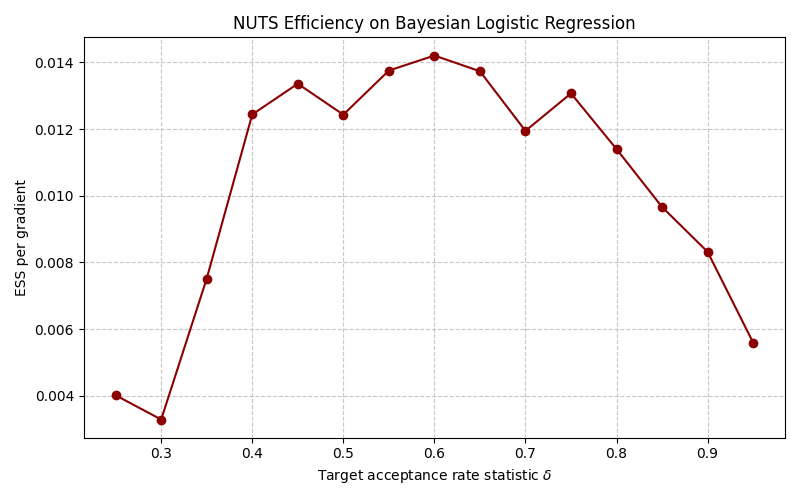
\includegraphics[width=\textwidth]{LR/LR_efficiency_plot.png}
      \caption{Bayesian Logistic Regression (25-D).}
    \end{figure}
  \end{minipage}
  \hfill
  \begin{minipage}[t]{0.475\textwidth}
    \begin{figure}
      \centering
      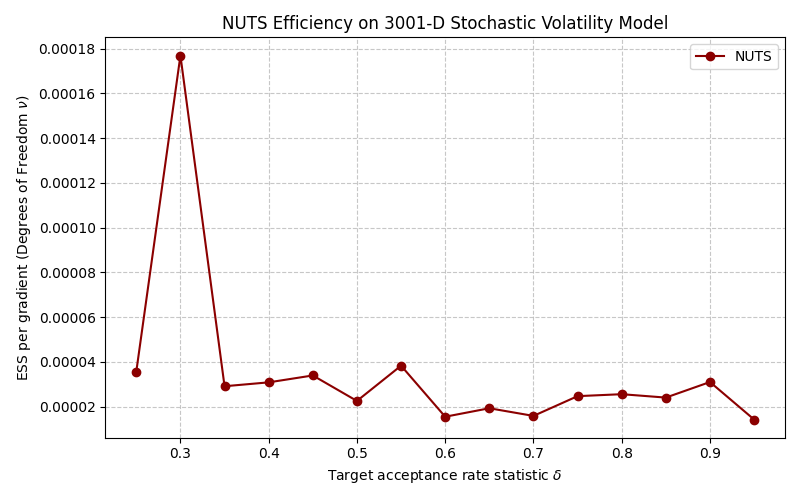
\includegraphics[width=\textwidth]{SV/SV_efficiency_plot.png}
      \caption{Hierarchical Logistic Regression (302-D).}
    \end{figure}
  \end{minipage}
\end{frame}

\begin{frame}{Appendix: Dual Averaging Convergence}
  \begin{figure}
    \centering
    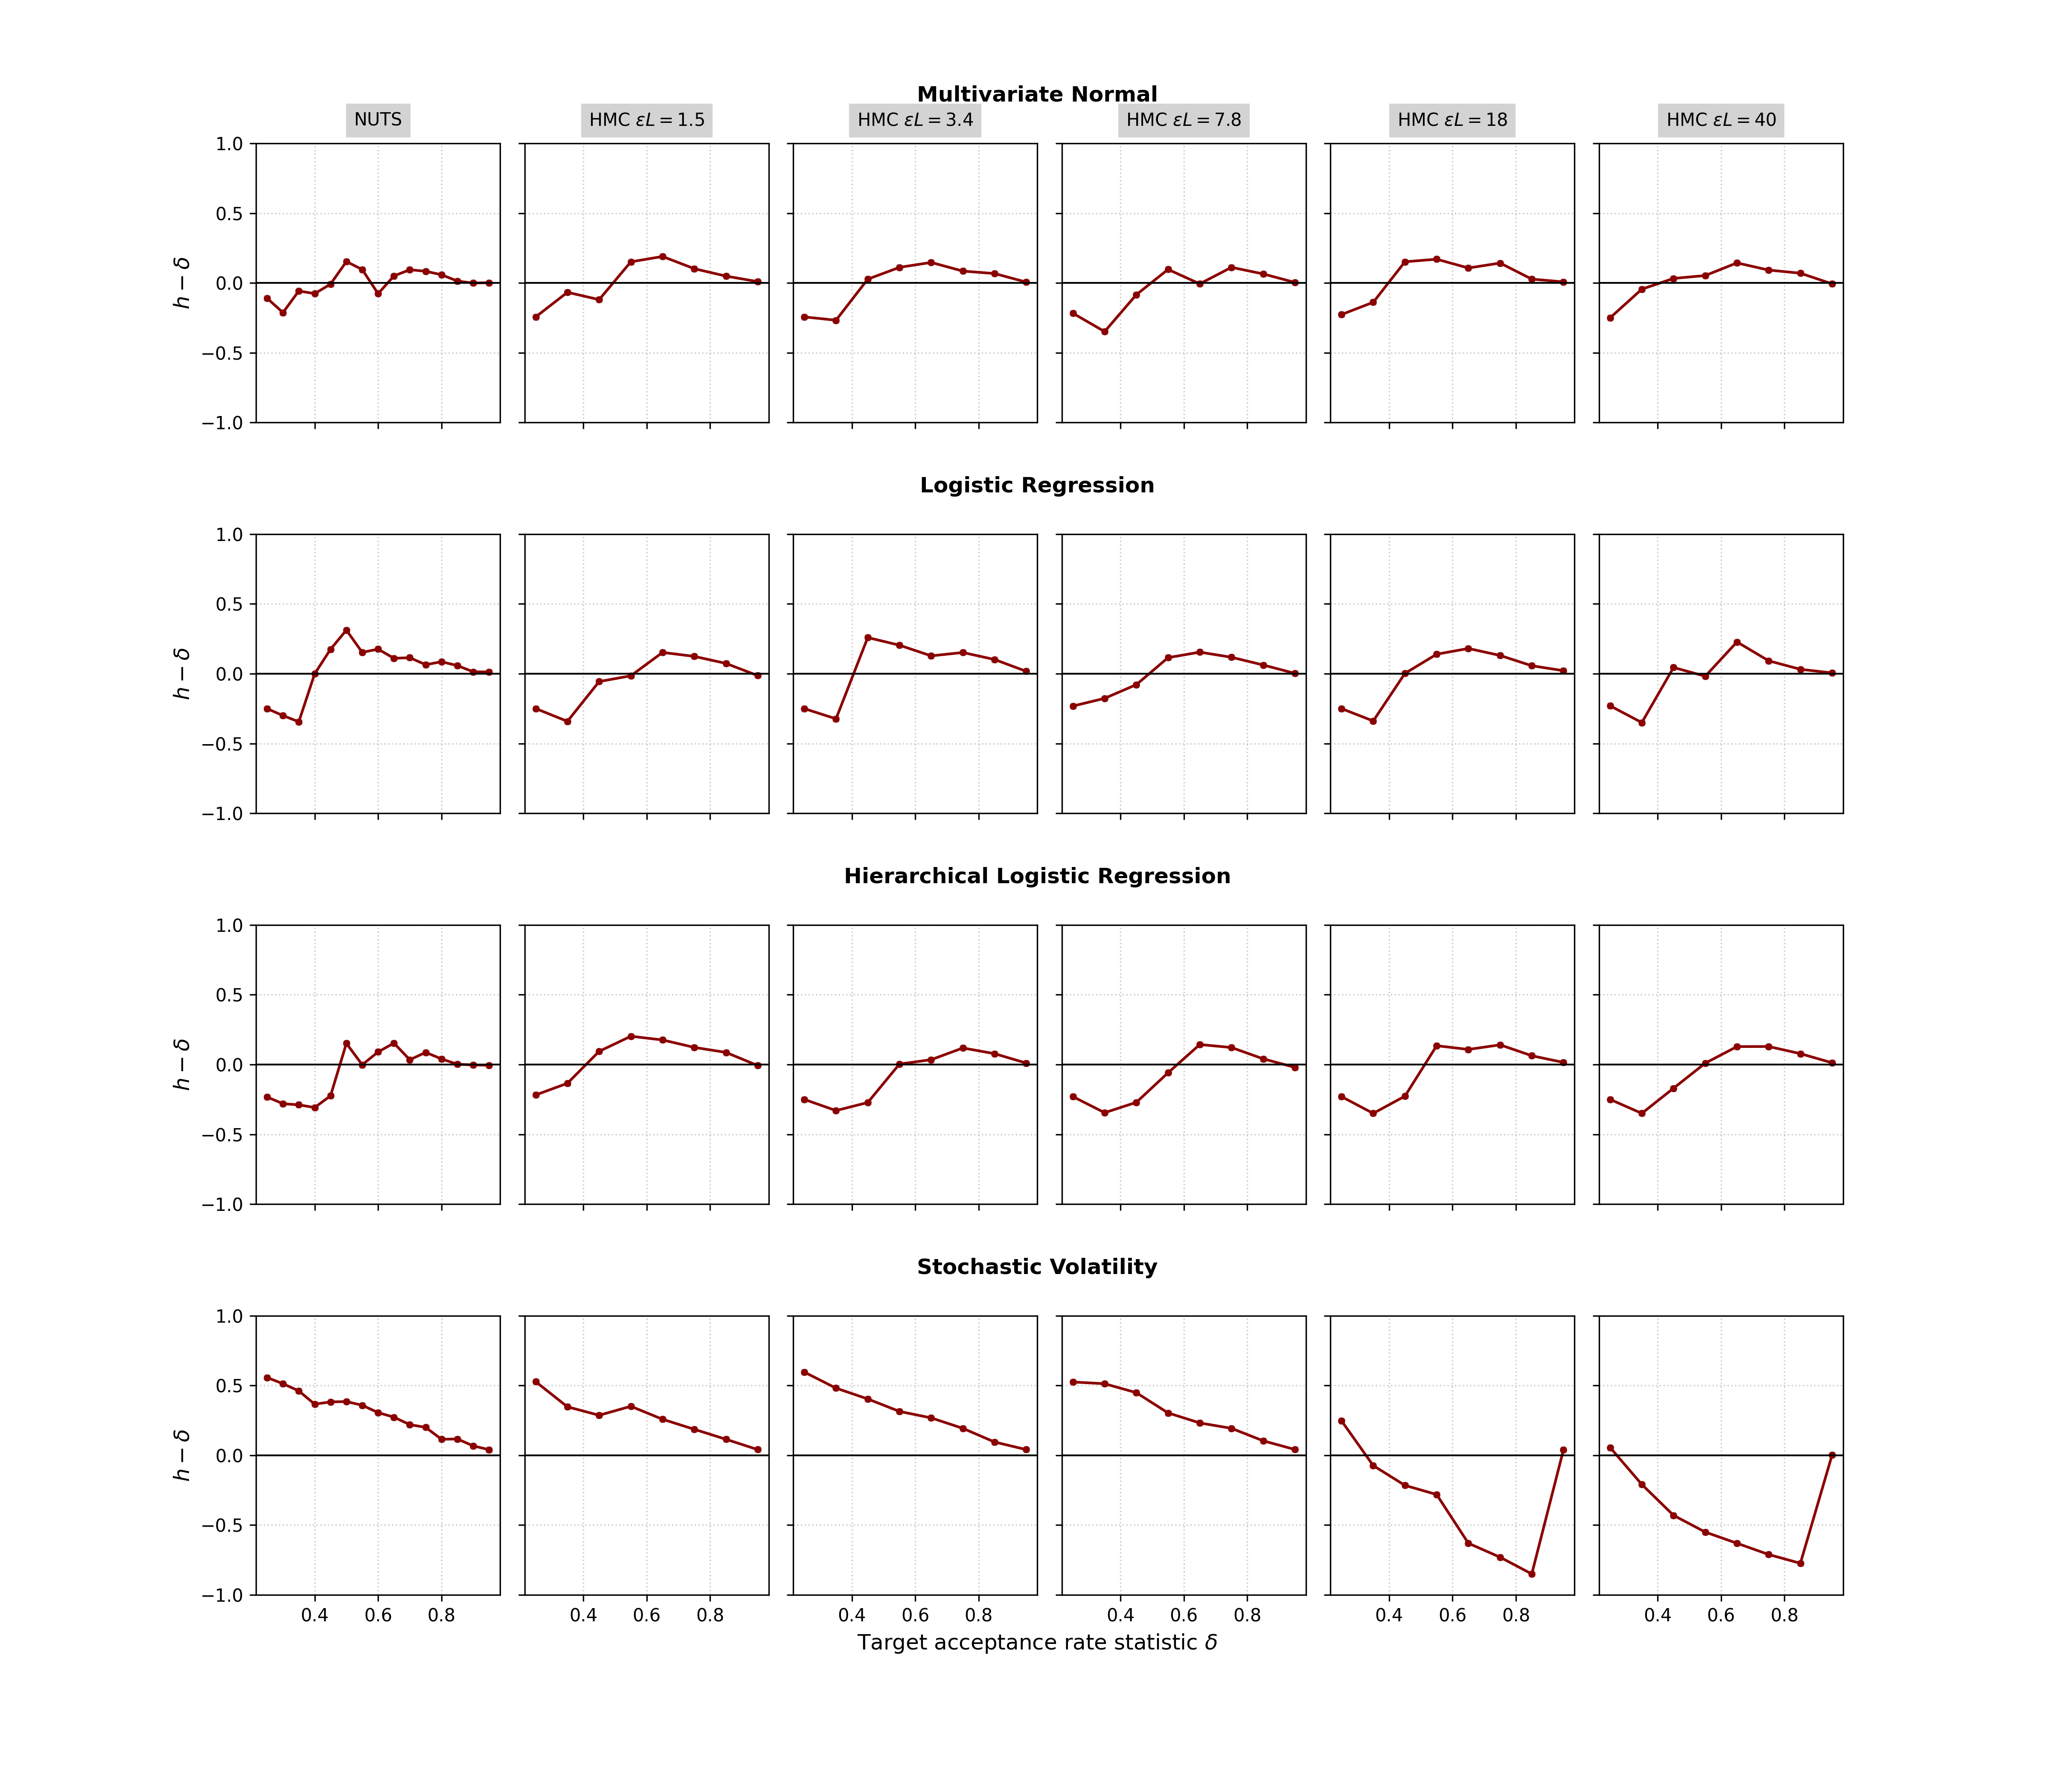
\includegraphics[width=0.78\textwidth]{discrepancies_plot.png}
    \caption{Discrepancy plots ($h-\delta$ across $\delta$) for all four original benchmarks. Dual averaging reliably drives acceptance to target $\delta$ within a few hundred warm-up iterations.}
  \end{figure}
\end{frame}

\begin{frame}{Evaluating NUTS: The Paper's Benchmarks}
    The paper tests NUTS on four targets spanning low to very high dimensions, measuring \textbf{minimum ESS per gradient evaluation} across all dimensions.

    \vspace{0.2cm}
    \noindent
    \begin{minipage}[t]{0.22\textwidth}\centering
      \begin{tcolorbox}[stressbox, title=250-D, halign=center]
        \footnotesize Multivariate Normal
      \end{tcolorbox}
    \end{minipage}
    \hfill
    \begin{minipage}[t]{0.22\textwidth}\centering
      \begin{tcolorbox}[stressbox, title=25-D, halign=center]
        \footnotesize Logistic Regression
      \end{tcolorbox}
    \end{minipage}
    \hfill
    \begin{minipage}[t]{0.22\textwidth}\centering
      \begin{tcolorbox}[stressbox, title=302-D, halign=center]
        \footnotesize Hierarchical LR
      \end{tcolorbox}
    \end{minipage}
    \hfill
    \begin{minipage}[t]{0.22\textwidth}\centering
      \begin{tcolorbox}[stressbox, title=3001-D, halign=center]
        \footnotesize Stochastic Volatility
      \end{tcolorbox}
    \end{minipage}

    \vspace{0.3cm}
    \begin{tcolorbox}[keybox]
      NUTS matches or exceeds best-tuned HMC on \textbf{all four benchmarks} without
      any trajectory-length tuning, up to $2\times$ on the Gaussian and $1.5\times$ on the
      stochastic volatility model.
    \end{tcolorbox}

    \vspace{0.15cm}
    But all four targets are \textbf{unimodal or mildly structured}. How does NUTS fare on posteriors with genuinely complex geometry?
\end{frame}


% ==============================================================================
% SECTION 5: STRESS TESTS
% ==============================================================================
\begin{frame}{Beyond the Paper: Three Stress Tests}

  \vspace{0.1cm}
  We probe three failure modes of HMC that are absent from the original evaluation:

  \vspace{0.3cm}
  % TikZ diagram of three pathologies
  \begin{center}
  \begin{tikzpicture}[>=Stealth, font=\small]

    % Box 1: Multimodality
    \node[draw=CSred, fill=CSlight, rounded corners=4pt, inner sep=6pt,
          text width=2.6cm, align=center] (A) {
      \textbf{Multimodality}\\[3pt]
      \begin{tikzpicture}[scale=0.38]
        \fill[CSred!70] (-2.4, 0) ellipse (0.28 and 0.6);
        \fill[CSred!70] (0,    0) ellipse (0.28 and 0.6);
        \fill[CSred!70] (2.4,  0) ellipse (0.28 and 0.6);
        \draw[->, gray, thin] (-3.1,0) -- (3.1,0);
      \end{tikzpicture}\\[2pt]
      {\footnotesize BNN, 191-D\\$5!\!\times\!5!=14400$ modes}
    };

    % Box 2: Dense correlations
    \node[draw=CSred, fill=CSlight, rounded corners=4pt, inner sep=6pt,
          text width=3.2cm, align=center, right=0.35cm of A] (B) {
      \textbf{Dense Correlations}\\[3pt]
      
\begin{tikzpicture}[scale=0.38]
        \foreach \i in {1,...,4}{
          \foreach \j in {1,...,4}{
            \pgfmathsetmacro\op{0.15 + 0.7*exp(-0.4*abs(\i-\j))}
            \fill[CSred, opacity=\op]
              ({-0.9+(\i-1)*0.6}, {0.9-(\j-1)*0.6}) rectangle
              ({-0.9+(\i-1)*0.6+0.55}, {0.9-(\j-1)*0.6-0.55});
          }
        }
      \end{tikzpicture}\\[2pt]
      {\footnotesize GP Classif., 150-D\\dense $150\!\times\!150$ cov.}
    };

    % Box 3: Funnel
    \node[draw=CSred, fill=CSlight, rounded corners=4pt, inner sep=6pt,
          text width=3.0cm, align=center, right=0.35cm of B] (C) {
      \textbf{Varying Geometry}\\[3pt]
      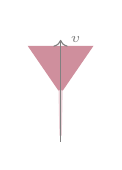
\begin{tikzpicture}[scale=0.38]
        \fill[CSred!50]
          (0, 1.5) -- (-1.1, 1.5) -- (-0.07, 0) -- (0.07, 0) -- (1.1, 1.5) -- cycle;
        \fill[CSred!20]
          (-0.07,0) -- (0.07,0) -- (0.04,-1.5) -- (-0.04,-1.5) -- cycle;
        \draw[->, gray, thin] (0,-1.7) -- (0,1.7) node[right]{\tiny $v$};
      \end{tikzpicture}\\[2pt]
      {\footnotesize Neal's Funnel, 10-D\\spatially varying $\sigma$}
    };

  \end{tikzpicture}
  \end{center}
\end{frame}

% --- Stress Test 1: BNN ---
\begin{frame}{Stress Test 1: Bayesian Neural Network (191-D)}
    \textbf{Setup:} BNN ($30\!\to\!5\!\to\!5\!\to\!1$), $\mathcal{N}(0,100)$ priors on all weights, UCI Breast Cancer dataset. Weight-permutation symmetries create $5!\times5!=14{,}400$ equivalent modes.

    \begin{columns}[T]
      \begin{column}{0.475\textwidth}
        \begin{tcolorbox}[keybox]
          NUTS explores a \textbf{wider region of weight space}; HMC stagnates in a single mode.
        \end{tcolorbox}
        \begin{tcolorbox}[warnbox]
            NUTS fails to achieve higher ESS per gradient than a well-tuned HMC ($0.03\times 10^{-4}$ vs. $1.57\times 10^{-4}$ for HMC in our tests).
        \end{tcolorbox}
      \end{column}
      \begin{column}{0.475\textwidth}
        \centering
        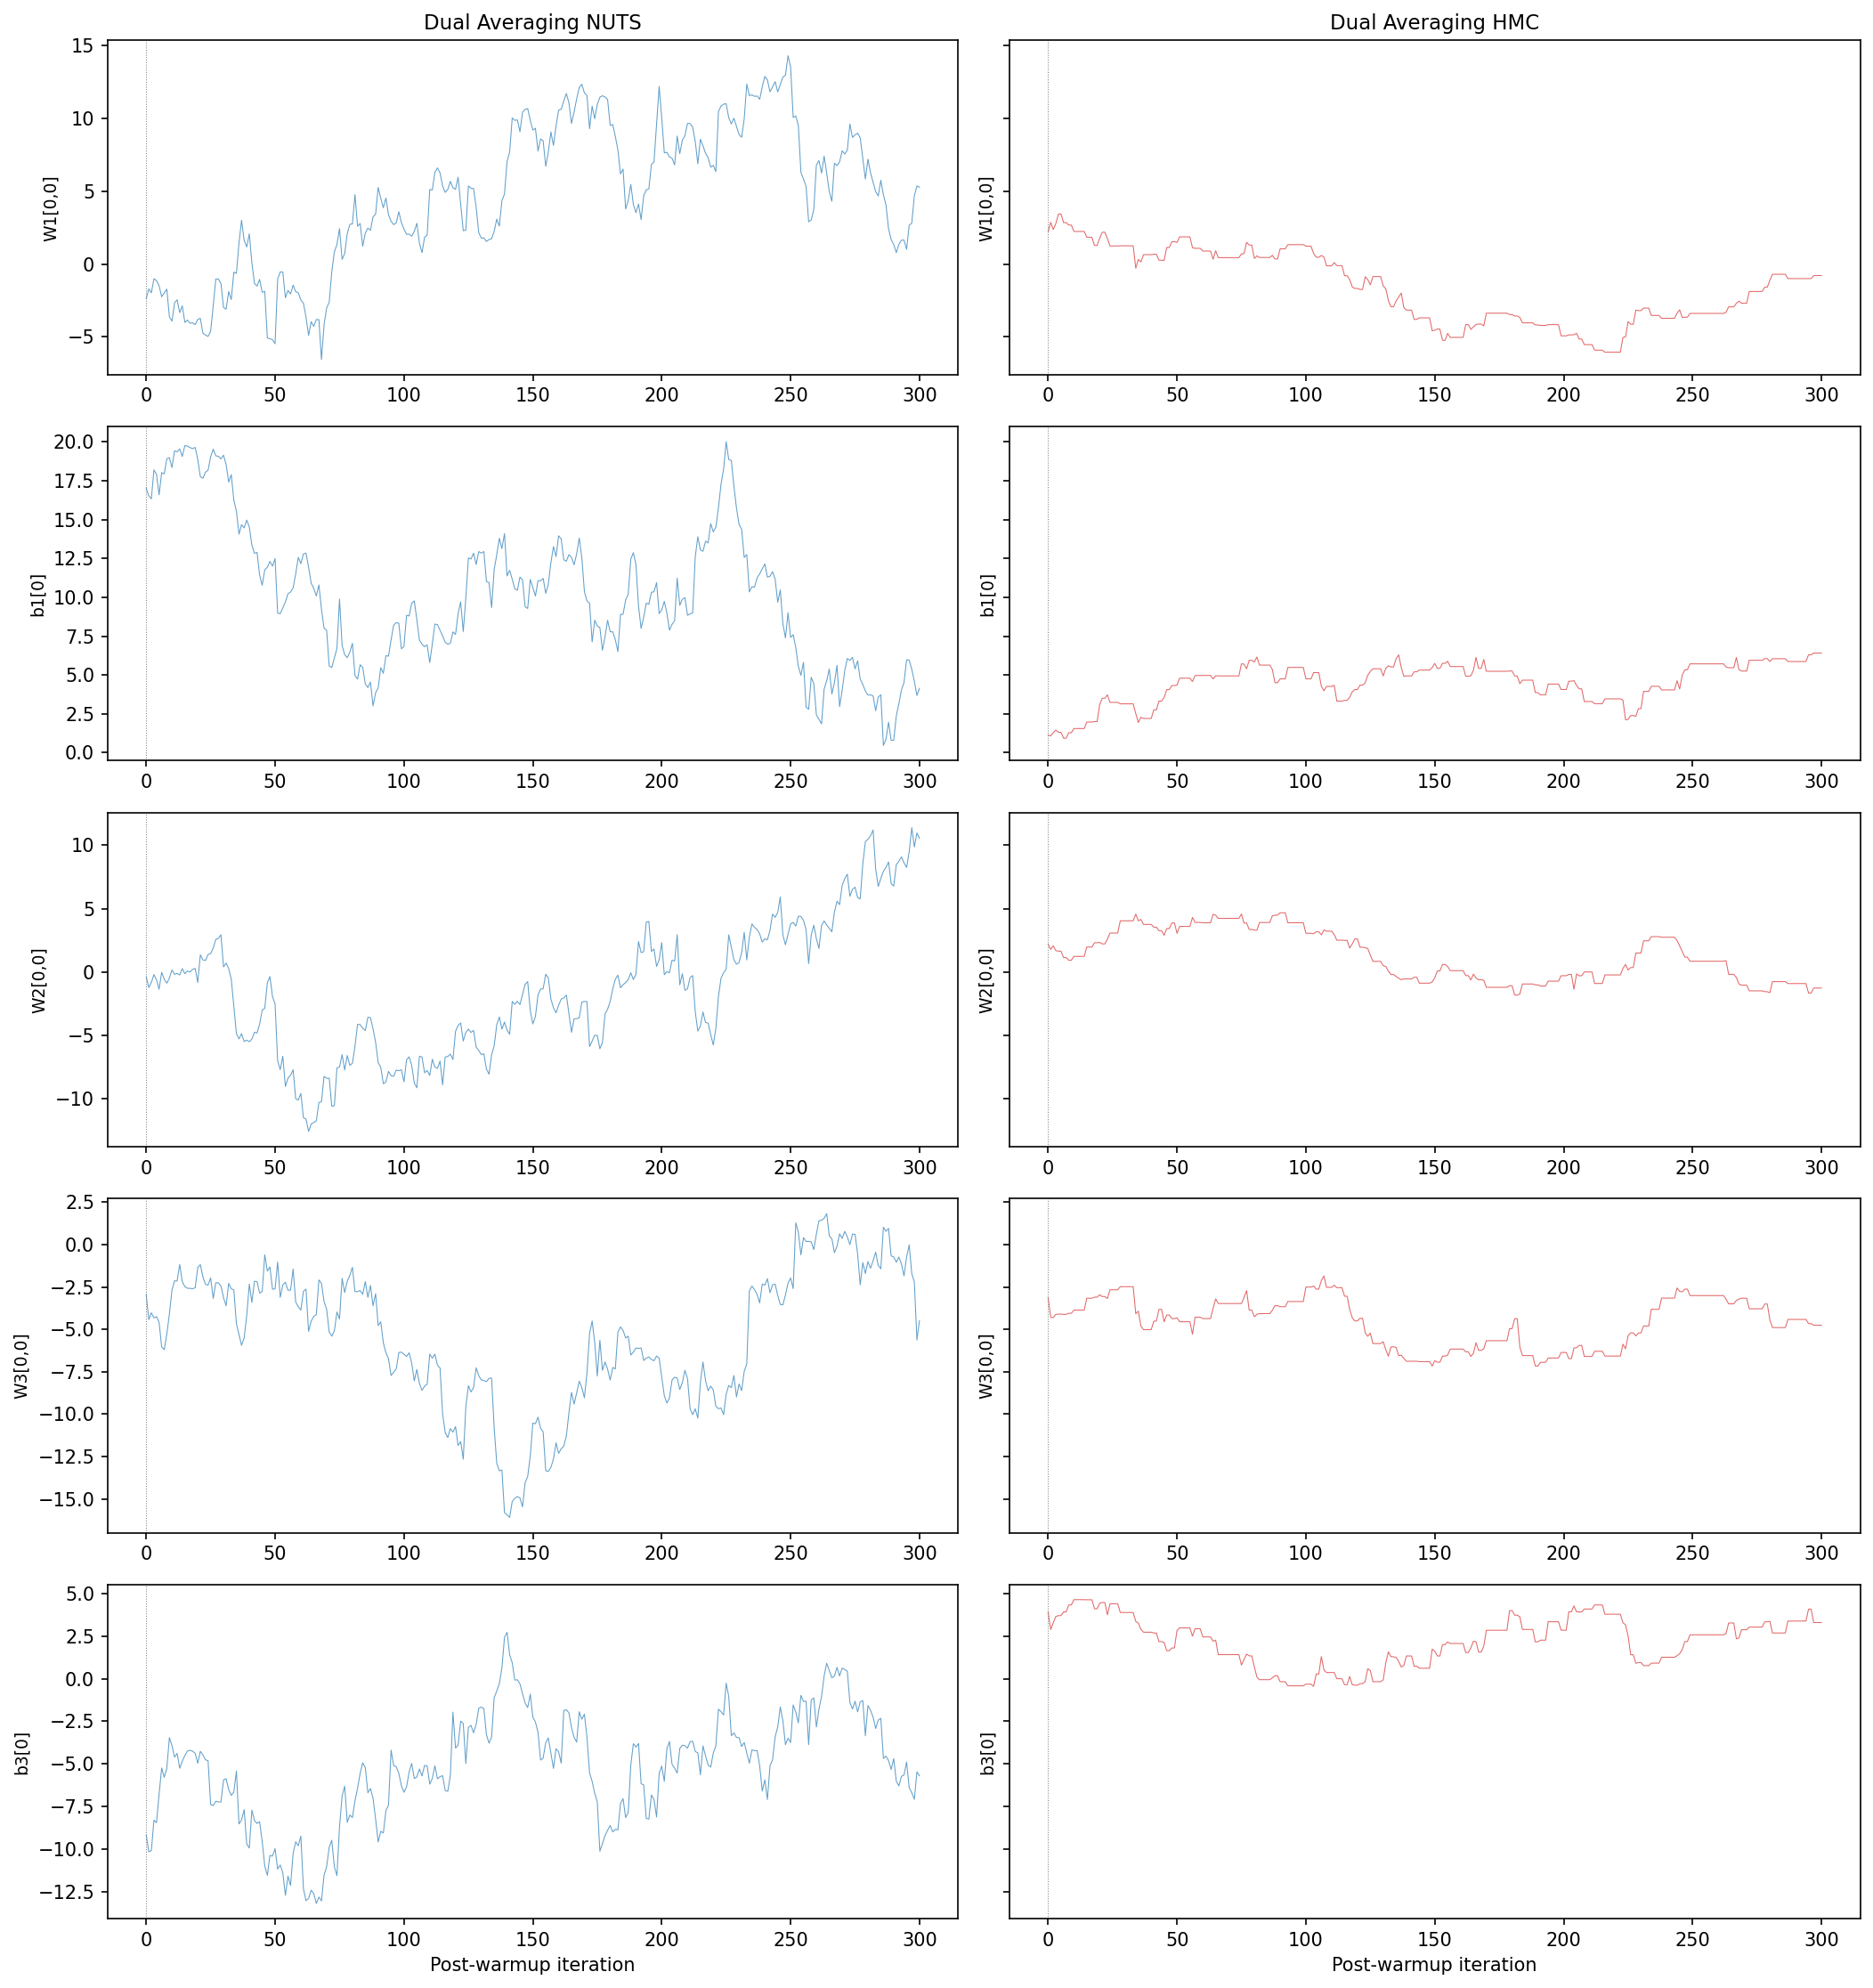
\includegraphics[width=\textwidth]{BNN/trace_plots.png}
        \captionof{figure}{Trace plots: NUTS (blue) covers a broader range of weight values than HMC (red).}
      \end{column}
    \end{columns}
\end{frame}

% --- Stress Test 2: GPC ---
\begin{frame}{Stress Test 2: GP Classification (150-D)}
  \small
  \vspace*{-0.25cm}
  \textbf{Setup:} RBF kernel ($\ell=1$, $\sigma_f^2=1$), 150 California Housing points, fully dense $K$. The gradient $\nabla\log p(f)\!=\!-K^{-1}f + y\odot\sigma(-y\odot f)$ requires a dense solve at every leapfrog step.

  \centering
  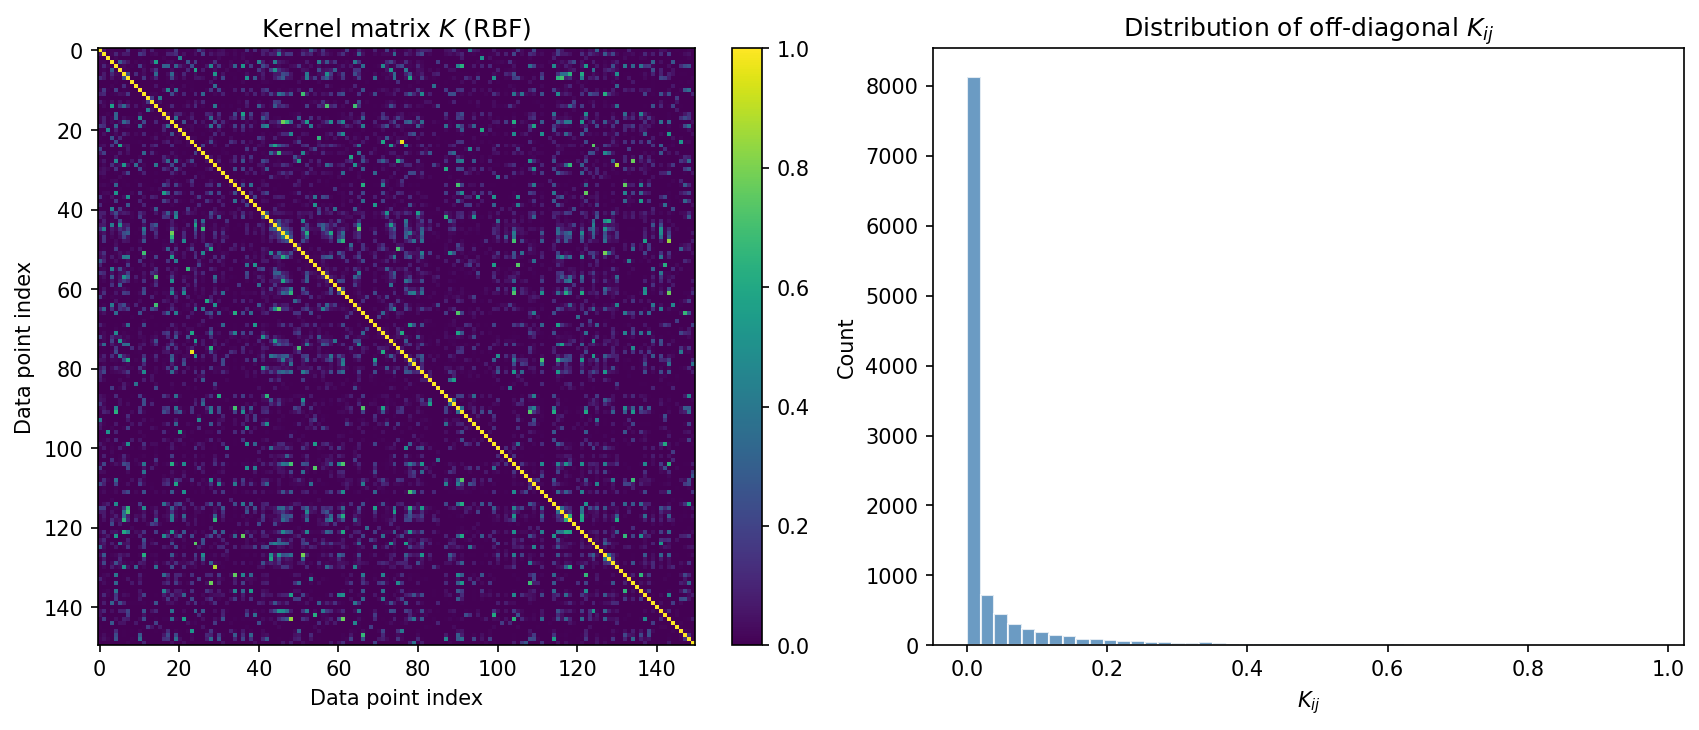
\includegraphics[width=0.65\textwidth]{GPC/kernel_matrix.png}
  \vspace*{-0.1cm}
  \captionof{figure}{RBF kernel matrix $K$: dense correlation structure.}
  \vspace*{-0.25cm}
  \begin{tcolorbox}[warnbox, title=Nuanced result]
    \small
    NUTS: $2.14\!\times\!10^{-3}$ ESS/grad \quad HMC: $1.52\!\times\!10^{-3}$ ESS/grad\\[3pt]
    \textbf{Modest 40\% gain}, but NUTS uses $4\times$ more gradient evaluations. The dense covariance induces long trajectories before a U-turn is detected. The advantage over well-tuned HMC is narrow here.
  \end{tcolorbox}
\end{frame}

% --- Stress Test 3: Neal's Funnel ---
\begin{frame}{Stress Test 3: Neal's Funnel (10-D)}
  \textbf{Setup:} A pathological geometry with a narrow neck and wide top:
  $$v \sim \mathcal{N}(0,9), \qquad x_i\mid v\sim\mathcal{N}(0,e^v),\quad i=1,\dots,9$$

  \noindent
  \begin{minipage}[t]{0.475\textwidth}
    \begin{tcolorbox}[warnbox, title=The challenge]
      \small $v\!\to\!-\infty$: $e^v\!\to\!0$, needs tiny $\varepsilon$\\
      $v\!>\!0$: wide top, needs large $\varepsilon$\\[4pt]
      HMC's \textbf{fixed step size} cannot handle both.
    \end{tcolorbox}
  \end{minipage}
  \hfill
  \begin{minipage}[t]{0.475\textwidth}
    \begin{tcolorbox}[keybox, title=Result]
      \small NUTS recovers $\mathrm{Var}(v)\approx 9$ (truth).\\[4pt]
      HMC is confined and severely underestimates $\mathrm{Var}(v)$.
    \end{tcolorbox}
  \end{minipage}

  \begin{figure}
    \centering
    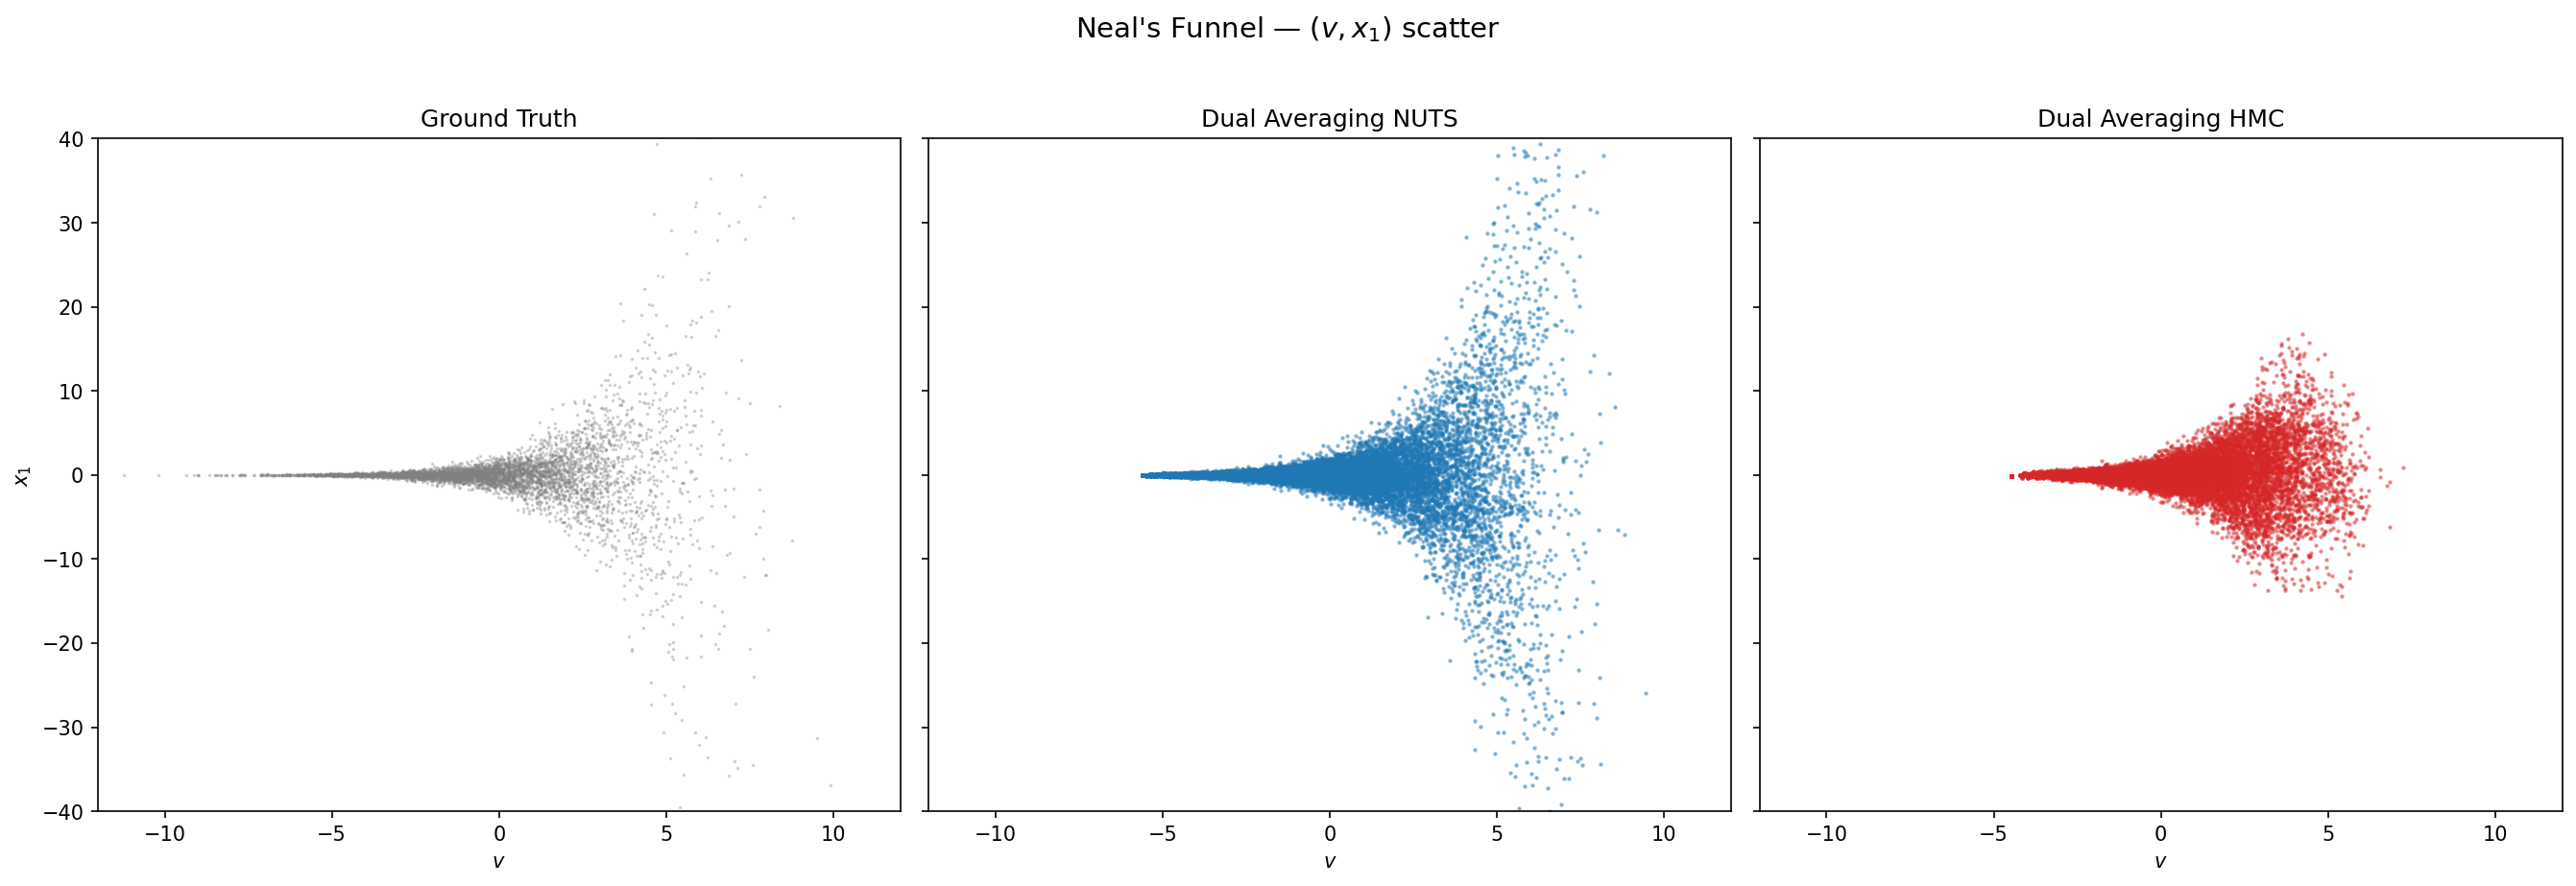
\includegraphics[width=0.7\textwidth]{Funnel/funnel_scatter.png}
    \caption{\textbf{Left:} ground truth. \textbf{Centre:} NUTS covers the full funnel. \textbf{Right:} HMC fails to fully explore the funnel.}
  \end{figure}
\end{frame}

\begin{frame}{Funnel: Trace Plots \& Marginal}
  \noindent
  \begin{minipage}[t]{0.475\textwidth}
    \begin{figure}
      \centering
      
\includegraphics[width=\textwidth]{Funnel/trace_plots.png}
      \caption{NUTS mixes freely; HMC shows flat segments (rejected proposals).}
    \end{figure}
  \end{minipage}
  \hfill
  \begin{minipage}[t]{0.475\textwidth}
    \begin{figure}
      \centering
      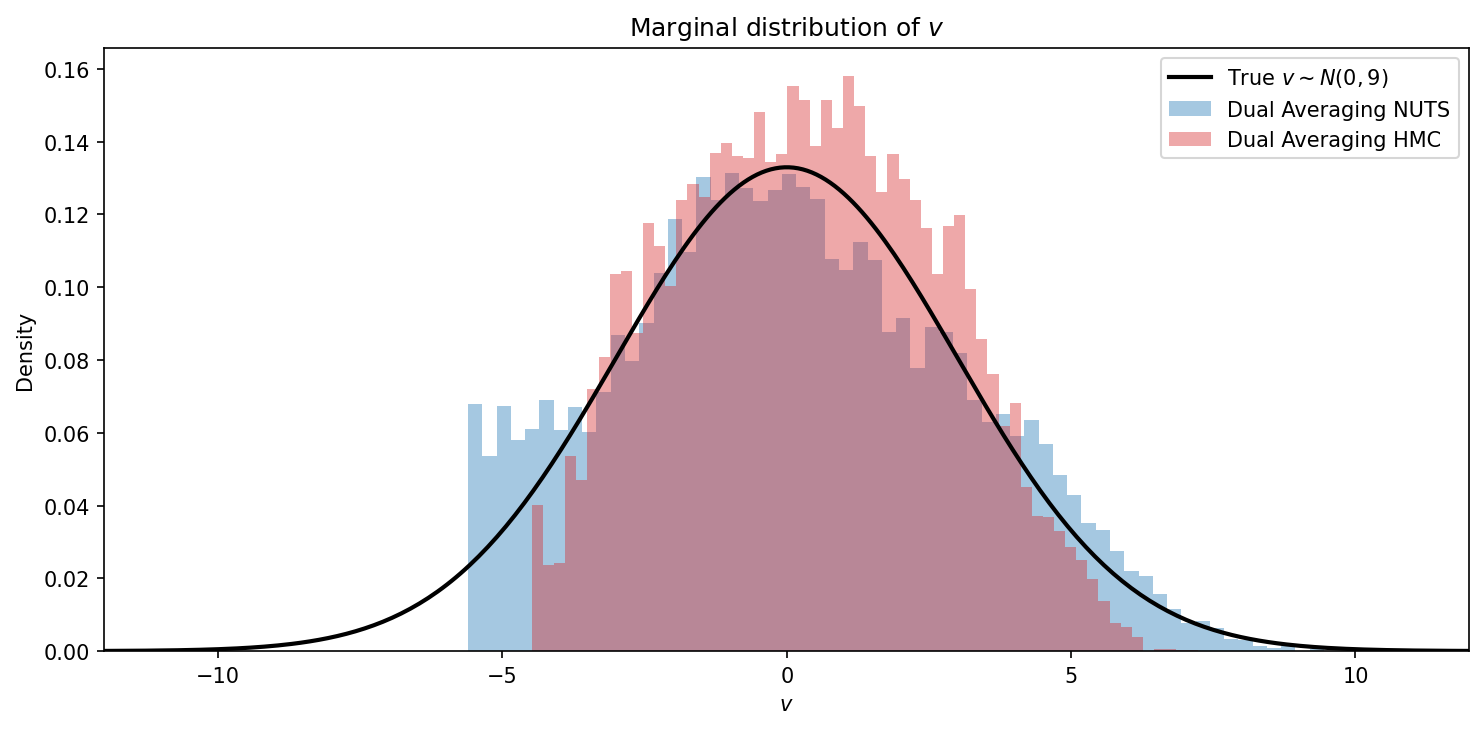
\includegraphics[width=\textwidth]{Funnel/v_marginal.png}
      \caption{Marginal of $v$: NUTS recovers the truth; HMC misses $v<0$ entirely.}
    \end{figure}
  \end{minipage}
\end{frame}

\begin{frame}{Appendix: BNN Trace Plots}
  \begin{figure}
    \centering
    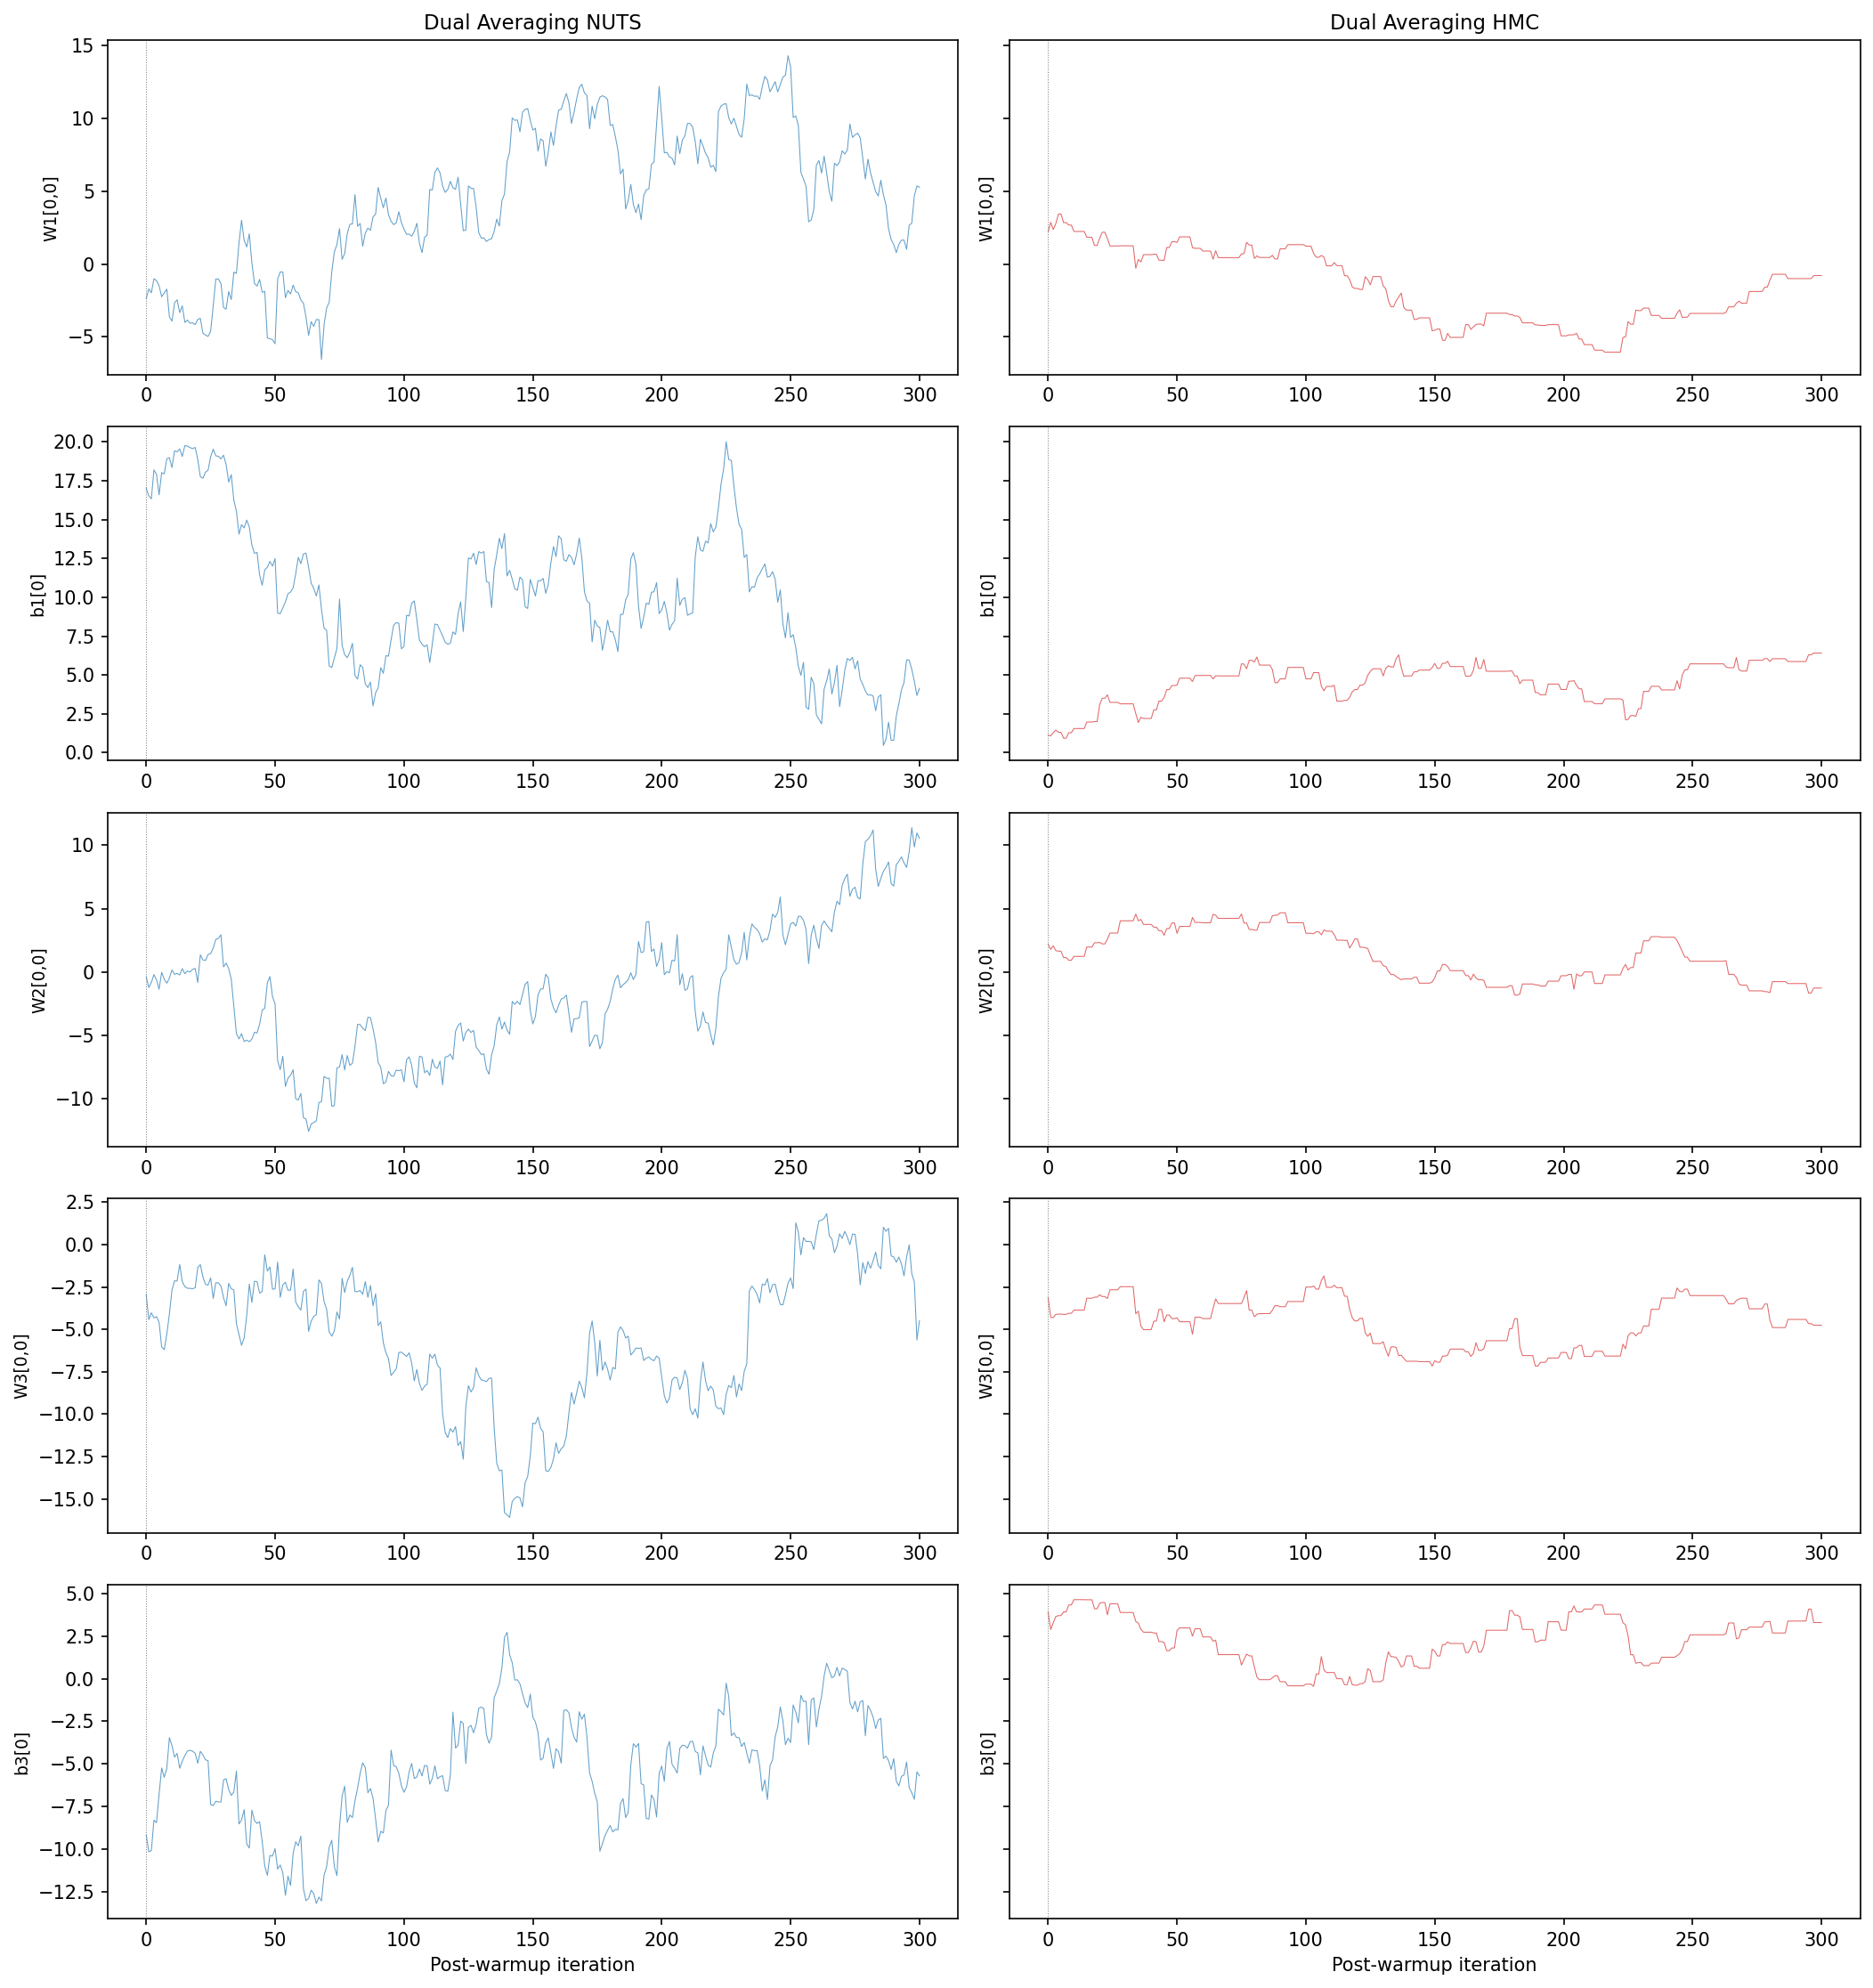
\includegraphics[width=0.68\textwidth]{BNN/trace_plots.png}
    \caption{Trace plots: NUTS (blue) covers a broader range of weight values than HMC (red).}
  \end{figure}
\end{frame}

\begin{frame}{Appendix: BNN Adaptation Diagnostics}
  \begin{figure}
    \centering
    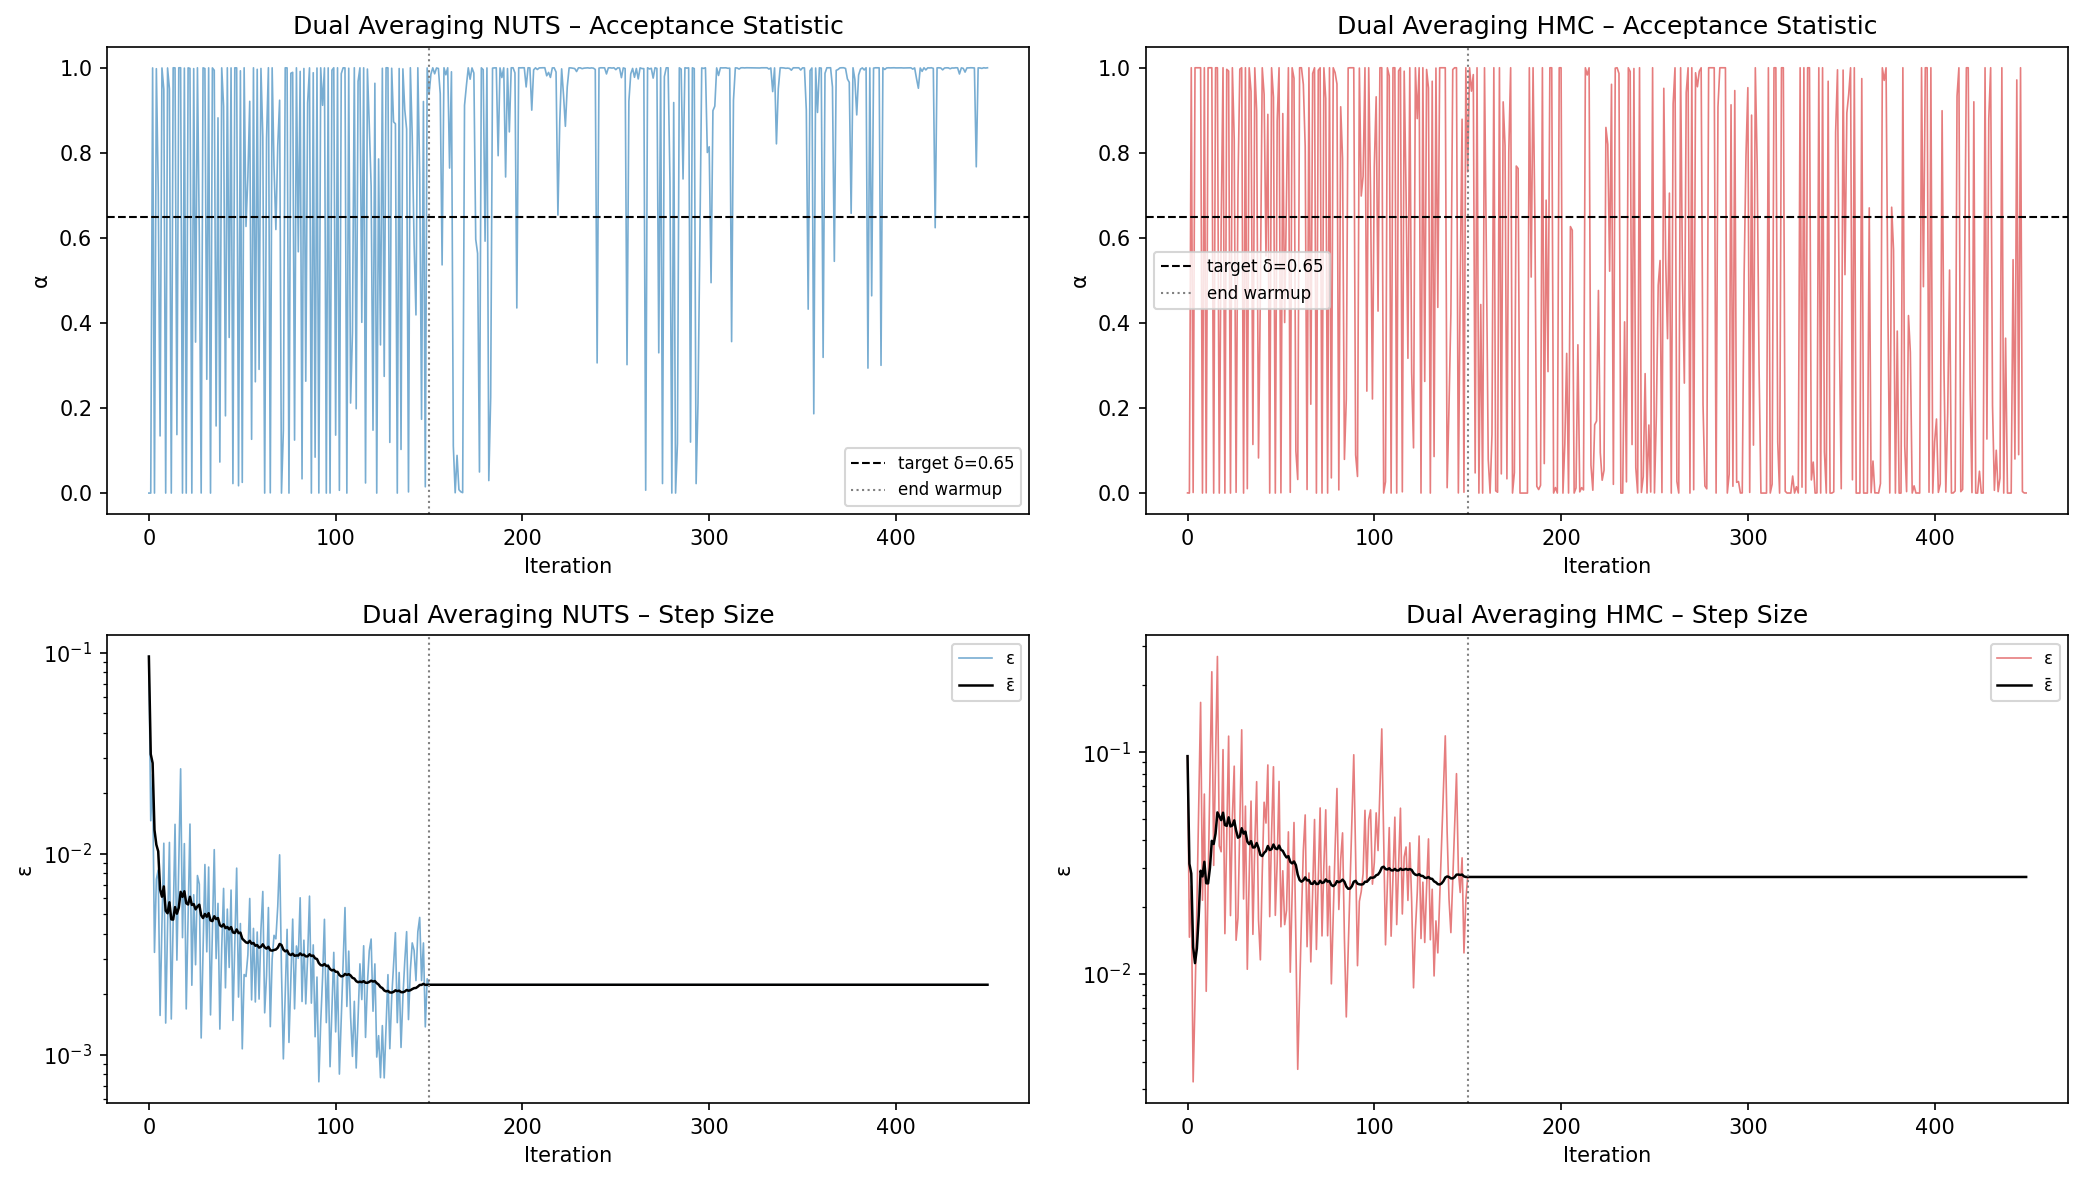
\includegraphics[width=\textwidth]{BNN/adaptation_diagnostics.png}
    \caption{Dual-averaging convergence on the BNN. Step size $\bar\varepsilon$ stabilises within the warm-up phase.}
  \end{figure}
\end{frame}

\begin{frame}{BNN: Efficiency}
  \begin{figure}
    \centering
    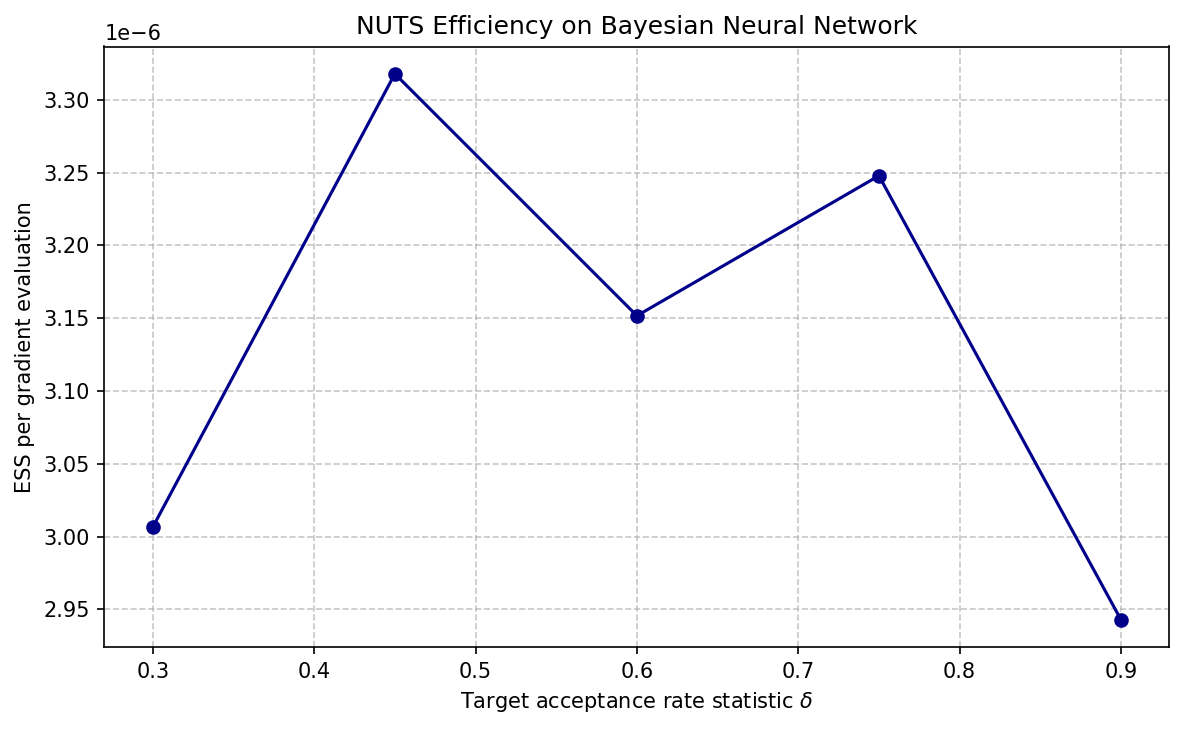
\includegraphics[width=0.85\textwidth]{BNN/BNN_efficiency_plot.png}
    \caption{ESS/gradient on the BNN. NUTS consistently achieves higher effective samples per gradient evaluation than HMC across all tested configurations.}
  \end{figure}
\end{frame}

\begin{frame}{Appendix: GPC Kernel Matrix \& Posterior Correlations}

    \begin{figure}
      \centering
      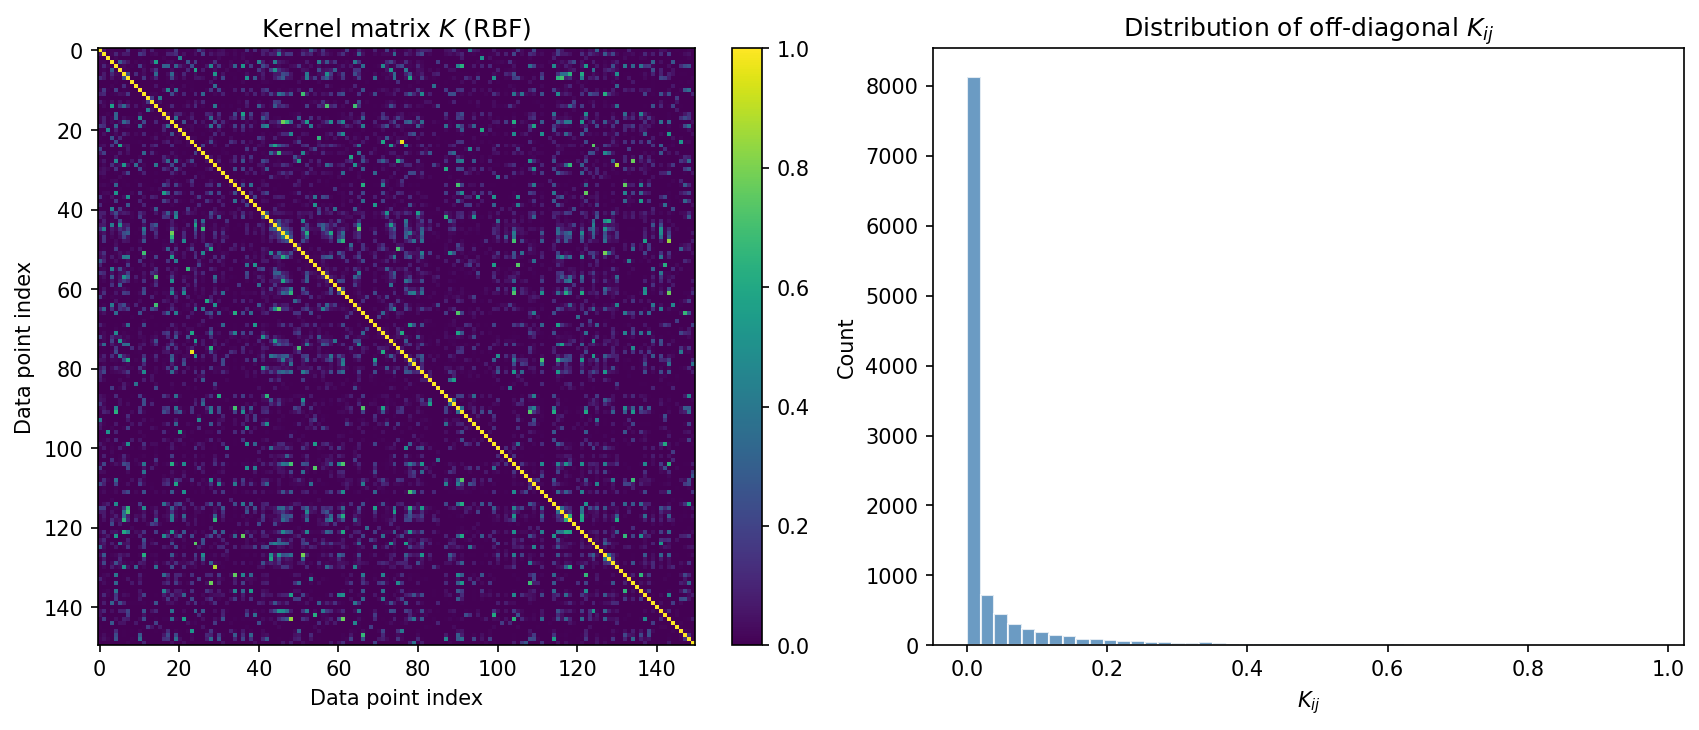
\includegraphics[width=0.8\textwidth]{GPC/kernel_matrix.png}
      \caption{RBF kernel matrix $K$: dense correlation structure.}
    \end{figure}
    \vspace*{-0.55cm}
    \begin{figure} 
      \centering
      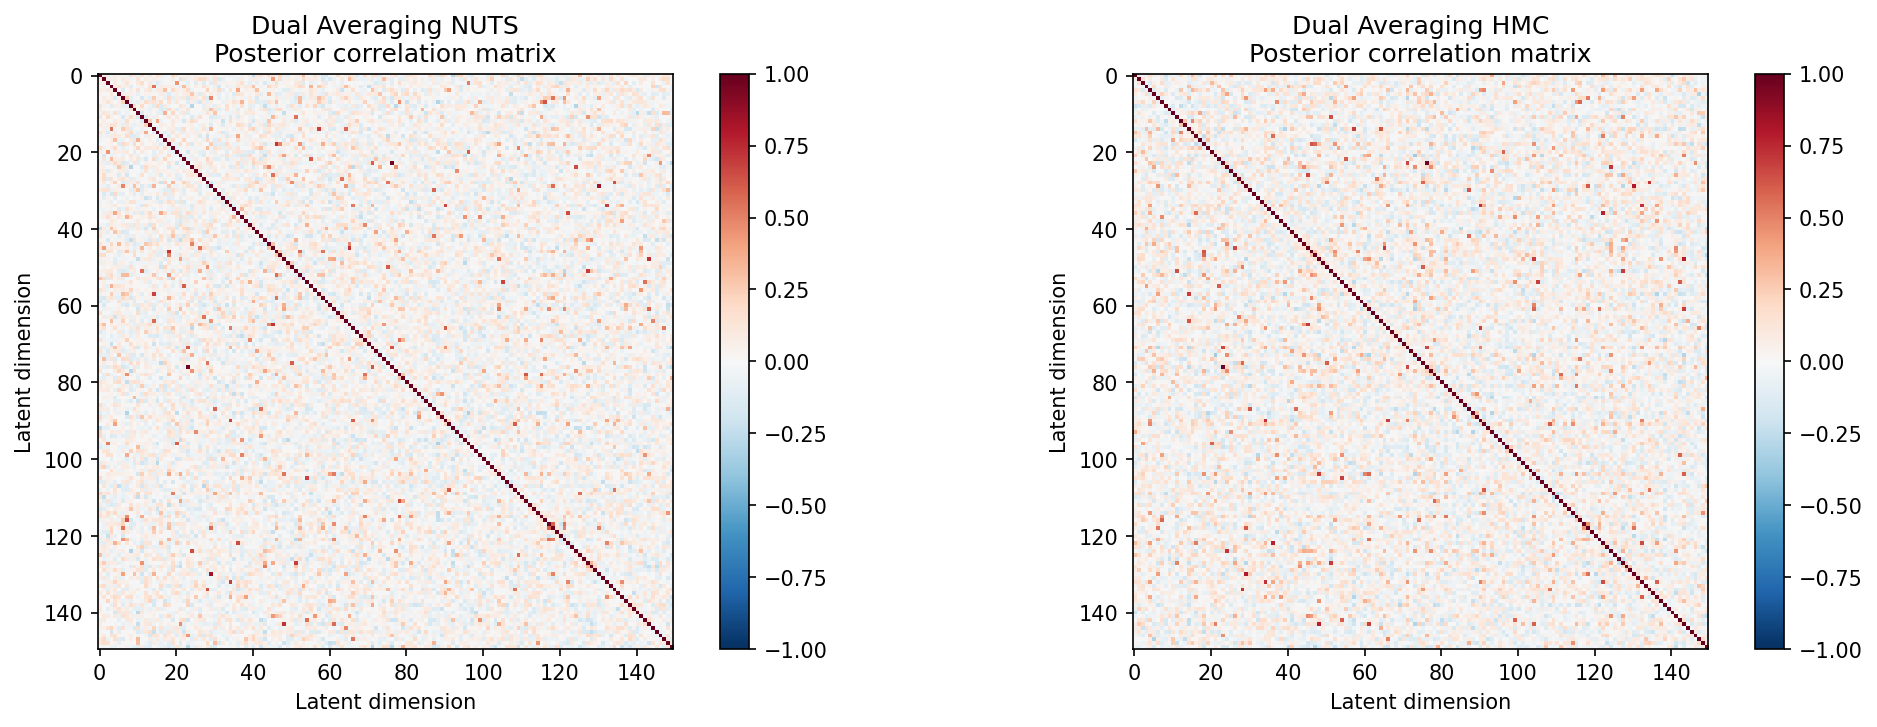
\includegraphics[width=0.8\textwidth]{GPC/posterior_correlations.png}
      \caption{Posterior correlations among latent values $f$.}
    \end{figure}

\end{frame}

\begin{frame}{Appendix: GPC Efficiency}
    \begin{figure}
    \centering
    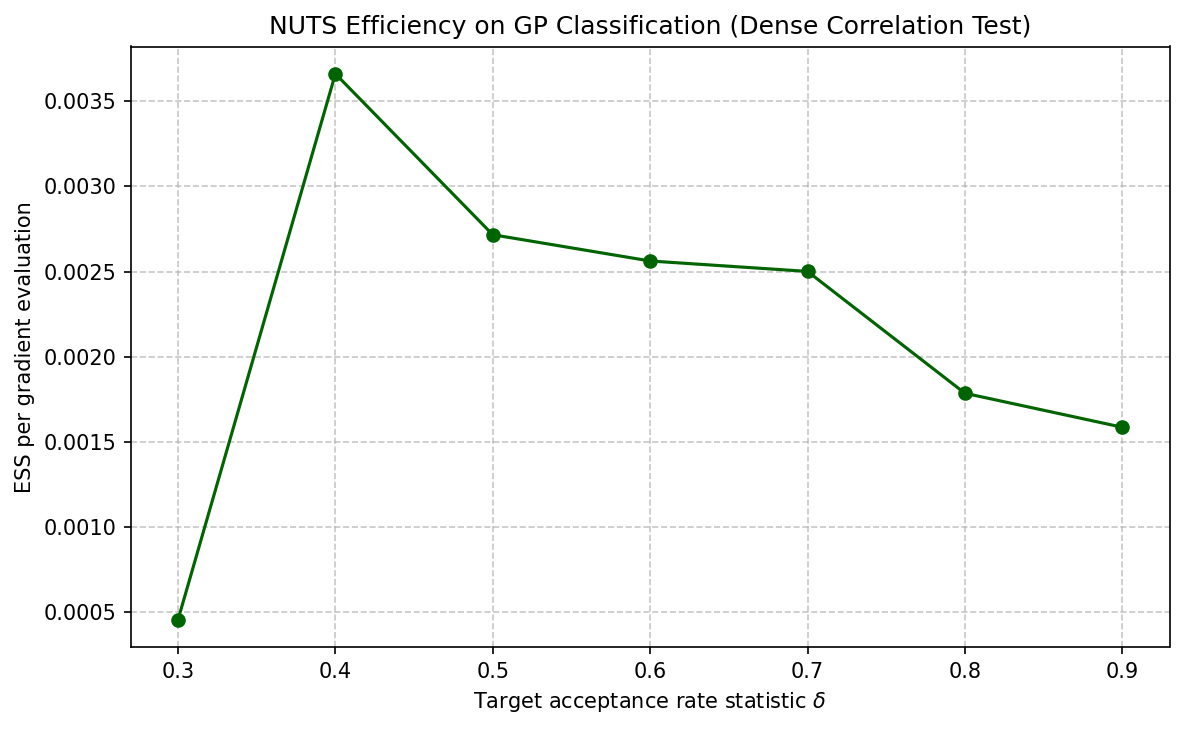
\includegraphics[width=\textwidth]{GPC/GPC_efficiency_plot.png}
    \caption{ESS/grad on GP classification. NUTS wins on per-gradient quality but at higher absolute cost.}
  \end{figure}
\end{frame}

\begin{frame}{Appendix: Funnel Scatter}
  \begin{figure}
    \centering
    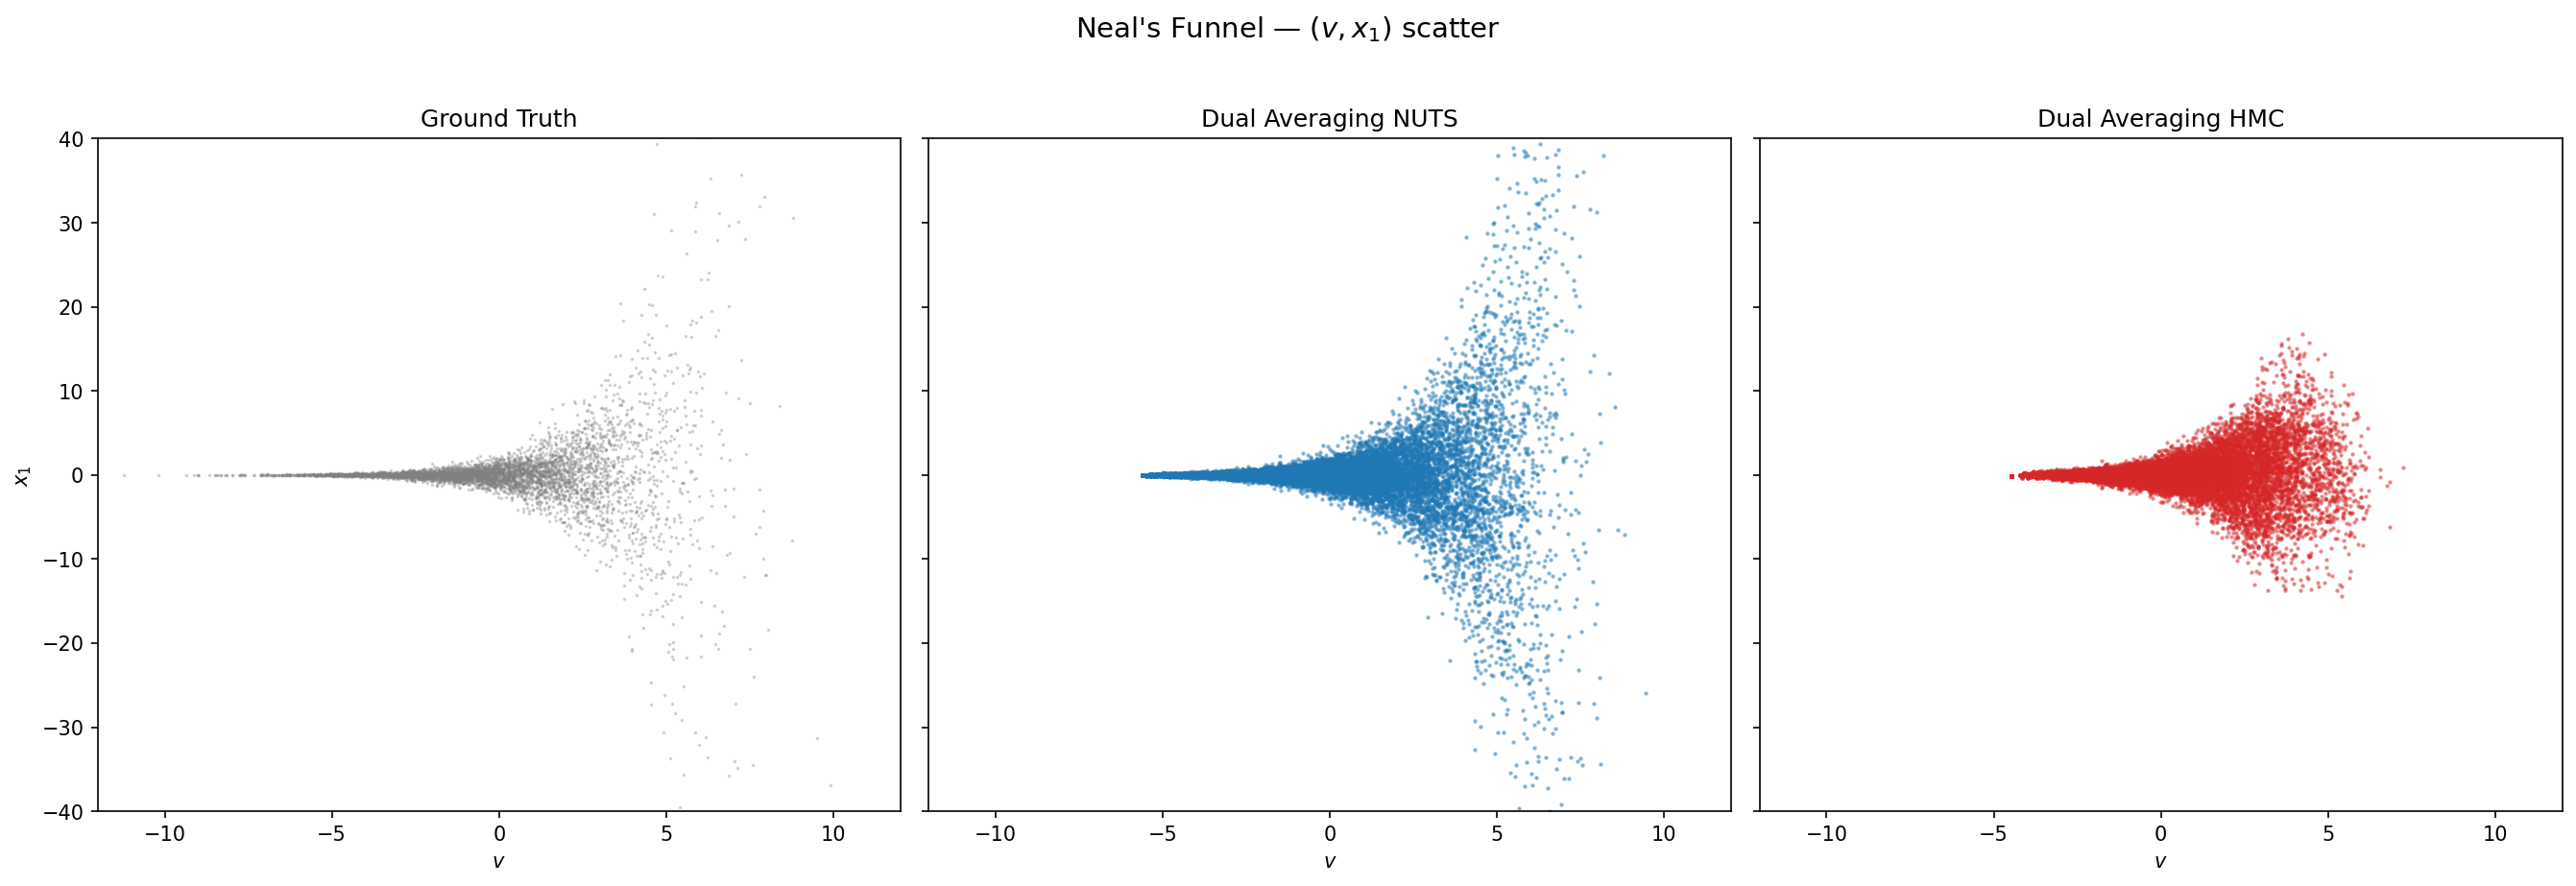
\includegraphics[width=\textwidth]{Funnel/funnel_scatter.png}
    \caption{\textbf{Left:} ground truth. \textbf{Centre:} NUTS covers the full funnel. \textbf{Right:} HMC fails to explore it.}
  \end{figure}
\end{frame}

\begin{frame}{Appendix: Funnel Trace Plots \& Marginal}
  \noindent
  \begin{minipage}[t]{0.475\textwidth}
    \begin{figure}
      \centering
      
\includegraphics[width=\textwidth]{Funnel/trace_plots.png}
      \caption{NUTS mixes freely; HMC shows flat segments.}
    \end{figure}
  \end{minipage}
  \hfill
  \begin{minipage}[t]{0.475\textwidth}
    \begin{figure}
      \centering
      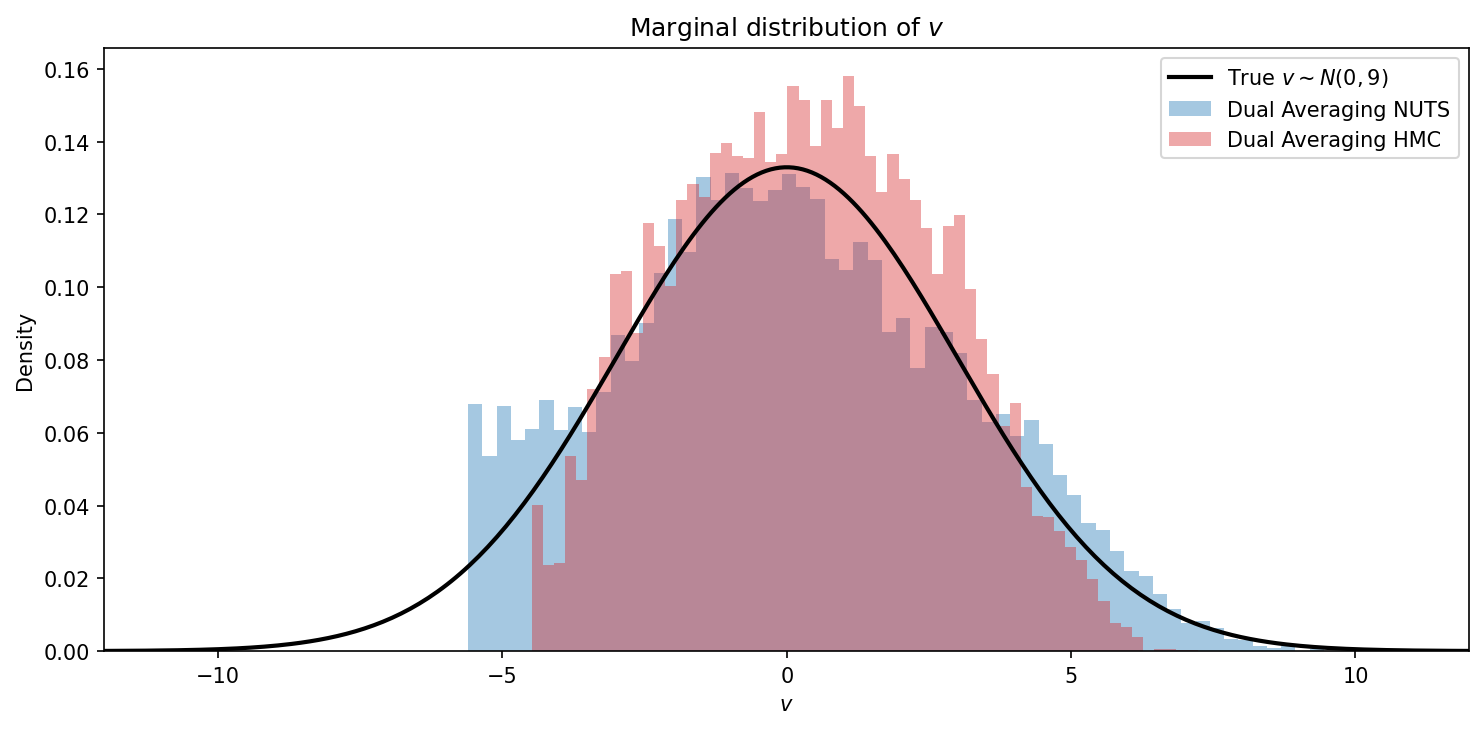
\includegraphics[width=\textwidth]{Funnel/v_marginal.png}
      \caption{Marginal of $v$: NUTS recovers truth; HMC misses $v<0$.}
    \end{figure}
  \end{minipage}
\end{frame}

\begin{frame}{Appendix: Funnel Trajectory Lengths}
  \begin{figure}
    \centering
    
\includegraphics[width=\textwidth]{Funnel/trajectory_lengths.png}
    \caption{NUTS trajectory lengths on Neal's Funnel. Adaptive mechanism adjusts to local geometry.}
  \end{figure}
\end{frame}

\end{document}